\chapter{Team 5 Agent Design}
\section{Game Specification}
Our agent represents an island that exists in the Archipelago where it interacts and collaborates with other islands (agents). All agents interact with a Common Pool of resources which is primarily used to facilitate governmental procedures and mitigate natural disasters that may occur (long-term collective risk dilemma). As a result of the short-term collective risk dilemma, there is not enough resources to satisfy all of agents but only enough to satisfice \textit{some} of them. According to \textit{Self-Organizing Multi-Agent Systems} by Pitts, satisfy means having all agent's needs taken care of. On the other hand, satisfice means only the basic needs/minimum requirements have been met. In this economy of scarcity, it may be sufficient that the agent's needs are satisficed. Each island presumably will have the objective of maximising its individual utility which requires collaboration with other islands.

In our implementation, the levels of resources held by our agent are divided into 'wealth tiers' which influence our agent's decision making strategies. Our interactions with other agents are driven by our \texttt{opinion} of them which evolves over time in the game. In every round, our agent computes its current wealth status and updates its opinion of others based on various factors explored below.

\subsection{Wealth Tiers}
We have defined four different wealth tiers and the respective thresholds to represent the status of the agent according to its current resources. The wealth tiers are defined as follows:
\begin{enumerate}
    \item \texttt{dying}: critical status. 
    \item \texttt{imperialStudent}: lower class (<30\% of starting resources).
    \item \texttt{middleClass}: middle class (<95\% of starting resources).
    \item \texttt{jeffBezos}: upper class (<200\% of starting resources).
\end{enumerate}

\subsection{Opinion Formation}
\label{subsec: opinion-formation}
\subsubsection{Design}
An opinion of other islands is our agent's general perception of them and is characterised by a \textit{general score} and a \textit{forecasting reputation}. Both are characterised by a score ranging from $1$ to $-1$, where $1$ represents the best possible perception of another island, and $-1$, the worst perception. A score of $0$ represents a neutral or indifferent opinion. We believe it is necessary to form opinions on more than one basis as opinion-oriented decisions may depend on different factors across various tasks. For example, it may happen that one agent is particularly stingy with gifting but is a very skilled forecaster. If our agent was then to decide which agents' forecasting data to trust, it would not make sense to exclude these agents on the basis of their stinginess, even though this may affect our propensity to share gifts with them in another part of the simulation.

While opinion formation is explored more in detail below, some potential events that may affect our opinion of other teams are as follows:
\begin{itemize}
    \item Allocating or distributing less than they initially offer for gifting.
    \item Giving allocation of common pool's resources to islands when holding the President role. 
    \item Sharing foraging information.
\end{itemize}

\subsubsection{Agent Implementation}
A structure has been implemented to provide the ability to potentially incorporate further attributes that influence our agent's opinion of others (each such attribute is termed an \texttt{opnionBasis} in the implementation). Current opinions are stored and updated in an \texttt{opinionMap} that is indexed by the IDs of other agents. Finally, a history of opinions per agents across turns is stored in an \texttt{opinionHistory} variable. This allows us to analyse how opinions evolve across time. The choice to include an opinion of our own agent in the aforementioned \texttt{opinionMap} was so the opinion of our agent can be adjusted based on the same measures that are used to form opinions of other teams. This allows for an interesting analysis how our agent performs given its own `behaviour’(essentially what our opinion of it would have been if it was another agent). Furthermore an addition parameter called "mood" was implemented into the agents behavior, mood directly affects how much the opinions of agents change by. When the agent is in \texttt{imperialStudent} tier opinion changes are magnified as the agent is under stress from the need to survive. Whilst if the agent is in the \texttt{jeffBezos} tier it is much more care free and his opinion will not change as much with useful or useless information. 

\section{Environment}
\subsection{Foraging}
\subsubsection{Design}
Our agent initially determines its foraging method through its wealth tier during the initial foraging turns (three turns which can be adjusted in agent configuration). The agent will attempt deer hunting if it is wealthy (\texttt{jeffBezos} tier) as deer hunting is a high risk foraging method with larger potential returns. Since the agent already has a large sum of money, a negative return is less significant in comparison to if it was poor. The agent will contribute a randomly selected amount between $20\%$ and $30\%$ of its wealth (changeable in the configuration). Whilst in the \texttt{middleClass} and \texttt{imperialStudent} tier it will only contribute $10\%$ to $20\%$ of its wealth. Furthermore, in the \texttt{middleClass}, the agent has the equal chance of either deer hunting or fishing. In the \texttt{ImperialStudent} tier, the agent will choose fishing as it is poor and needs to avoid risk to survive. Finally when we are in the dying tier, at risk of dying in three turns, we invest all our money into fishing in hopes that we can catch at least a single fish and make it out of the dying tier. After every round the agent stores all its past experiences in its foraging history in addition to other agents past experiences if they were shared.  

Our agent executes the following steps to determine its foraging method:
\begin{itemize}
    \item First it enters \texttt{InitialForage()}) as described above.
    \item After the initial foraging it proceeds to do \texttt{normalForage()}) which is based off the foraging history stored from the initial turns. The agent first looks to find the best foraging method using (\texttt{bestHistoryForaging()}).
    \item \texttt{bestHistoryForaging()} First looks at the foraging history and calculates the average Return on Investment (RoI) its entire foraging history which is calculated using:
    \\  \begin{center} $\dfrac{output}{input}-1$ \end{center}
    \item In the case that the average RoI is less than 0 for both methods (no profit) then it returns none which indicates that there is no best foraging method. Otherwise it set the best foraging method as the one with the highest average RoI. 
    \item If the average RoI is above 0 then the agent assigns a probability of $10\%$ (set in configuration) to switch to either hunting or fishing.
    \item Afterwards, it looks at the number of hunters in the previous three turn (set in configuration). From this it will decrease the random probability of selecting deer hunting, the amount it decreases will depends on how close to the current turn the hunter went hunting. The closer to the current turn the lower the chances to hunt, additionally it also looks at the number of deer caught, if no deer were caught then the chances will not decrease. This can be seen in Table~\ref{table:Probability Avoiding Deer Hunting} . The number of deer caught would be halved and multiplied into the the probability.
           {\begin{table}[]
                 \begin{center}
                 \caption{Probability table of avoiding deer hunting according to the number of hunters in the past 3 turns (with scaled version (0.035))}
                 \label{table:Probability Avoiding Deer Hunting}
                        \begin{tabular}{|c|c|c|c|c|c|c|c|c|}
                        \hline
                                                 &   & \multicolumn{3}{c|}{Turns before current   hunt} &         & \multicolumn{3}{c|}{Turns before current   hunt scaled} \\ \hline
                                                 &   & 3                  & 2             & 1           & Scaling & 3                  & 2                & 1               \\ \hline
                        \multirow{6}{*}{Hunters} & 1 & 0.333333           & 0.5           & 1           & 0.035   & 0.011667           & 0.0175           & 0.035           \\ \cline{2-9} 
                                                 & 2 & 0.666667           & 1             & 2           & 0.035   & 0.023333           & 0.035            & 0.07            \\ \cline{2-9} 
                                                 & 3 & 1                  & 1.5           & 3           & 0.035   & 0.035              & 0.0525           & 0.105           \\ \cline{2-9} 
                                                 & 4 & 1.333333           & 2             & 4           & 0.035   & 0.046667           & 0.07             & 0.14            \\ \cline{2-9} 
                                                 & 5 & 1.666667           & 2.5           & 5           & 0.035   & 0.058333           & 0.0875           & 0.175           \\ \cline{2-9} 
                                                 & 6 & 2                  & 3             & 6           & 0.035   & 0.07               & 0.105            & 0.21            \\ \hline
                        \end{tabular}
                \end{center}
            \end{table} }  
    \item The probabilities to switch foraging methods are summed and applied to the method with the highest average RoI, resulting in the foraging method of choice
\end{itemize}

Now that our agent has decided its method of foraging, it needs to determine the amount of resources to contribute
\begin{enumerate}
    \item In the case the best foraging method is none where no RoI was positive:
        \begin{itemize}
            \item The agent will skip foraging for one turn.
            \item If the agent has already skipped last turn, then it is forced to forage as there is a need to get resources to survive. It will randomly select the foraging method and enter double the amount of resources it would normally invest (10\% to $20\%$) with, in hopes it could catch at least a single fish or deer.
        \end{itemize}

    \item In the case a method has positive RoI:
        \begin{itemize}
            \item It look at the input that gave the best RoI for that foraging method in addition to the method that gave the best profit.
            \item Then it takes a percentage of both best RoI and best profit, and added a random amount from ±$5\%$ of its total resources as its contribution.
            \item Looking at the number of islands alive, it then increases its contribution the less islands that are alive. This is to avoid contributing insufficient resources when other islands die and we are unable to reach the threshold to catch any animals. 
            \item Finally it restricts our contribution to a maximum of $40\%$ of our wealth.
        \end{itemize}
\end{enumerate}

Our agent's general opinion of others is heavily affected by the information available from other agents, thus if other agents refuses to share their foraging data, our agent will also stop sharing foraging data and have a lower opinion of them as well. \newline


\textbf{Future Works}\newline 
In future implementation, it would be interesting to investigate the application of machine learning techniques for the following tasks:
\begin{itemize}
    \item Determining the optimal foraging method or location if multiple foraging zones are implemented.
    \item Determining the best way to communicate with other agents in a way that may influence their foraging behaviours to benefit our agent.
\end{itemize}

\section{Inter-island Governmental Organisation (IIGO)}
\subsection{Common Pool}

The agents can request resources from the common pool, get their allocation and contribute to the common pool. The overall intention of each agent is to maximize utility and thus, our agent tries to estimate each legitimate claim in every round and ask for the highest possible allocation amount that would be accepted by the President. Additionally, there are some specific scenarios that our agent seeks for more resources than it "deserves" because it is low in resources. In these critical scenarios, the agent not only asks for more but also tries to steal from the common pool and does not contributes to it, to assure its survival. Thus, the strategy of our agent is shaped as follows: \newline

The agents requests for the permission from the President to take resources from the common pool and the President replies with the allocation amount. The requested amount depends on the \textit{turn}, the \textit{wealth status} of our agent and the \textit{allocationHistory} from the President. if \textit{allocationHistory} indicates approval of allocation amount of the President in the latest turn, the agent will request a higher amount of resource compare to the said allocation amount in \textit{allocationHistory}. However, if the President refused to allocate any resource to the agent lately, the agent will request a minimum amount to survive, which is $30\%$ of the initial resources given to an island, when it needs help from the common pool.


Every turn, our agent will decide if it can or needs to take any resource from the common pool. Ideally, the amount of resources taken from the common pool should be equal to the allocation amount given by the President. However, that is only true when our agent is doing well regarding financial status, \texttt{middleClass} or above. When the agent is in poor financial state, it will try to take the minimum amount necessary to survive, even if it exceeds the amount approved by the President. \newline

The agents are asked to contribute an amount of resources for tax. In the ideal circumstances, our agent will contribute at least the minimum amount of tax to the common pool to help funding IIGO operations. However, when our agent is in a poor state, below \texttt{middleClass}, it will ignore tax until it can get back on its feet once again. \newline

Our agent also contributes to the common pool to help the community. The important factor that decides if our agent will contribute or not is the flow of resource in the common pool since the last turn. If the flow is negative, it indicates that the trend of roles and other agents is to spend more than to contribute to the common pool. In that case, our agent will not make any contribution to the common pool. However, if the contribution is higher than the spending, our agent will contribute $1/6$ of the positive flow of resources to the common pool to assist the community. Unfortunately, if our agent in a poor financial state, it will ignore this contribution until it can get back to the normal state. \newline

Beside contributing to help the community, our agent also tries to use the common pool for disaster mitigation. This contribution is determined based on our disaster forecast's \textit{magnitude}, \textit{epicentre}, \textit{period}, \textit{confidence interval},  and the agent's current \textit{wealth}. From these values, an ideal contribution amount will be calculated. The confidence interval indicates the ideal amount of resource to contribute to the common pool. It is done this way to ensure our agent does not waste a lot of resources in case of uncertain predictions. In cases where predictions were made with higher certainty, the agent will want to ensure that the damage is mitigated when the incident happens. The ideal contribution is proportional to the damage and inversely proportional to the distance between the island and disaster's epicentre. Our agent will only contribute $20$\% of the ideal contribution $1$ day before the disaster may hit. The other $80$\% will be given on the day of the predicted disaster. This is to ensure that the purpose of the contribution (mitigating disaster) will be preserved. And since disaster occurs after IIGO events, it is acceptable to donate most of the resources on the day of the disaster. In cases where our agent's resources is not sufficient to match the calculated amount above, it will contribute $50$\% of its current resources for the purpose of mitigating the disaster. \newline

\subsection{Opinion Formation in Common Pool Transactions}
Our agent looks at how the the allocation has been given by the President and updates its opinion score with respect to the agent acting as the President. This helps form positive perception to President who tries to support fellow agents whenever having the mean to. The opinion score changes as follow:



\begin{itemize}
    \item If there is no allocation from the President even when there's sufficient amount in the common pool, it will cause a negative effect to opinion score.
    \item If the allocation is less than what was requested, there will be a light negative effect to opinion score.
    \item If the President approves an allocation amount equal to greater than the requested amount, there will be a positive effect to opinion score. 
\end{itemize}

\subsection{Sanction Payments}
Sanction are imposed when an agent breaks the rules such as stealing from the common pool. Since ignoring sanction payment will lead to longer sanction period, our agent will always pay the entire sanction amount as long as it has enough of resources. 

\subsection{Monitoring Roles} 
Our agent decides whether or not to monitor roles based on its opinion towards the client holding office. It is done this way because monitoring requires resources from the common pool and unnecessary monitoring will take the resources away from those who need it most. Furthermore, our agent's opinion is formed based on how interactive and supporting the other agents are towards fellow agents, thus it is a reasonable metric to use.

\subsection{Future Work}
Currently, the salary and actual spending of IIGO roles are not public to the agents. It would be a huge improvement to analyse the flow of resources in the common pool. The decision to contribute to the community through common pool will be more fair if those values are published. \newline

At the moment, the amount of contribution for mitigating disaster purpose is calculated based on only our agent's forecast. the model will improve a lot if the function takes into account predictions shared from other teams also. However, the agent may put a heavier weight on its prediction to make sure its not being tricked into contributing to the common pool for other purposes. 


\section{Inter-island Trade Organisation (IITO)}
\subsection{Gifts}
\subsubsection{Design}
Due to the short-term collective risk dilemma that is foraging, it is in the best interest of all the agents to keep other agents alive. Thus, not only does our agent requests for gifts but also offers gifts to others depending on its \textit{wealth tier}, the \textit{balance of resources} over the last turn and its \textit{opinion} towards the other agent. To form a well-rounded opinion and decide on the optimal strategy, our agent keeps track of the gift history and continuously updates its general opinion towards the others once it receives gifts. \newline

In the case that our agent is in \texttt{jeffBezos} or \texttt{middleClass} wealth tiers, it will assist other agents. The amount our island can give is limited to a percentage of its total resources which scales according to the wealth tier, the higher the wealth tier the greater the percentage as the agent has an abundance of resources. If our agent is in \texttt{imperialStudent} tier, it can partially assist agents that are in critical condition, however it will look to keep its resources for survival. Thus, it will not give any gifts to agents that are not in critical condition or have a low opinion of. Whilst, if our agent is in \texttt{Dying} status it can barely survive so it does not have the luxury to offer other agents resources. For the same reason, it does not request from islands that are in \texttt{Critical} status.  \newline

Our agent stores all of its gifting history to modify its opinion on other agents and act based on this. In more detail, when our agent has a positive opinion towards another agent it attempts to maximise their satisfaction and offers them an amount equal to what they requested for, depending on the wealth tier our agent is in . The higher the wealth tier the close our agent offers what was requested. In contrast, if they have a negative opinion it takes less consideration of their requests and more of what our agent wants to offer. All of the requests are limited to a certain percentage of our resources which is dependant on our wealth tier. \newline

Overall supporting other agents is beneficial in the long run, as the more agents that survive the more likely they can mitigate greater risk of the long-term Collective Risk Dilemma. By offering to the others, when our agent has the capacity to do so, our agent attempts to make them have positive views towards it. This is advantageous as other agents are likely to assist our agent when in need, with either gifts or assistance when they occupy one of the three government roles. Furthermore, when our agent is in lower wealth tiers it reduces the offers to other agents and focus on its own survival regardless of others opinions on our agent.

\subsubsection{Role of opinions in gifting}
More specifically, our agent stores previous gift history in \texttt{giftHistory} the gift history holds:
\begin{enumerate}
    \item What it requested; What was offered to it; The amount it accepted with the reason and The actual received amount.
    \item What they requested for; What our agent offered them; The amount they accepted with the reason and What they actually received.
\end{enumerate}

In each turn, our agent adjusts its opinion towards the others using a method called \texttt{giftOpinions}:
\begin{itemize}
    \item Negative Effect: Received less than offered.  
    \item Slight Negative Effect: Offered less than requested.
    \item Slight Negative Effect: If they requested the most compared to the others.
    \item Slight Positive Effect: Received more than they offered.
    \item Slight Negative Effect: If they requested the least compared to the others.
    \item Positive Effect: Received more than requested.
\end{itemize}

To calculate the request amount our agent uses a function called \texttt{GetGiftRequests} which requests gifts, in the the \texttt{jeffBezos} Tier,  from all other agents that are not in Critical state to maximise our utility. Depending on our wealth tier and opinion of other agents the amount requested will vary, requesting less from agents with higher opinion scores. To calculate the amount our agent offers, there is a function called \texttt{GetGiftOffers} which takes into consideration the requested amount from each team and returns a counter offer according to their opinion level and our wealth tier. The function \texttt{GetGiftResponses} obtains the response offer that we get from other teams and accepts all the offers that were give to our agent as there is no reason to decline gifts that could benefit our agent no matter the amount. \newline

{\textbf{Future Works}}\newline
Currently, the higher the opinion we have the less we request from an island. However, the a unique dynamic could be implemented where if the agent can meaning that we would be exploiting the positive relationship with our highly rated islands, asking for more. Furthermore, we could have looked into the amount of resources that islands were giving us in total to further adjust how we grade our opinion of them. 

\section{Inter-island Forecast Organisation (IIFO)}

IIFO implementation covers making disaster predictions/forecasts based on a history of disaster observations and predictions from other teams. 

\subsection{Basis of Forecasts}
The forecasting implementation generates forecasts based on several factors as explored below.

\subsubsection{Experience}
Most importantly, we use our past observations of disasters that occurred in \texttt{disasterHistory} to inform our current and future forecasts. Forecasts attempt to predict the following characteristics of a disaster:
\begin{enumerate}
    \item\textbf{(x,y) co-ordinates} of disaster epicentre.
    \item \textbf{magnitude} (severity) of disaster.
    \item \textbf{period} - the time (number of turns) between successive disasters. For a given forecast, this will involve predicting the time until the next disaster.
\end{enumerate}

One effective way to capture this notion of experience is to estimate the probability distribution function (pdf) of the underlying process that generates these disasters. However, given that agents are not provided any knowledge of these distribution functions, they can only make estimates using sample data collected through their interaction with the environment. Given that agents have no \textit{a priori} knowledge about distribution types, parametric estimation methods such as MLE (maximum likelihood estimation) are not suitable. Instead, kernel density estimation (KDE) was employed to estimate the pdf of each forecast variable (as listed above). KDE is a non-parametric approach to estimating a pdf and does not require any knowledge about the type of distribution. For a univariate iid sample $x_1, x_2, \dots, x_n$ and unknown pdf $f$, the KDE estimate $\widehat{f}$ is given by Equation~\ref{eq: KDE Estimate}.

\begin{equation}
\widehat{f}_{\gamma}(x)=\frac{1}{n} \sum_{i=1}^{n} K_{\gamma}\left(x-x_{i}\right)=\frac{1}{n \gamma} \sum_{i=1}^{n} K\left(\frac{x-x_{i}}{\gamma}\right)
\label{eq: KDE Estimate}
\end{equation}

where $K$ is the non-negative kernel function with bandwidth $\gamma$. While many different kernels may be used, a Gaussian kernel was exclusively used in this implementation. The bandwidth represents the width of each Gaussian "hump". Larger bandwidths result in a larger degree of smoothing. The literature details a few mechanisms for selecting an appropriate bandwidth based on data, and in this implementation, the Scott rule-of-thumb method was used. The details thereof are not included for the sake of brevity.

The KDE estimates for a normal distribution for varying numbers of samples using our implementation is shown in Figure~\ref{fig:KDE_uniform} below. Naturally, the estimated pdf more closely resembles the underlying counterpart with an increasing number of samples.

\begin{figure}[!htb]
    \centering
    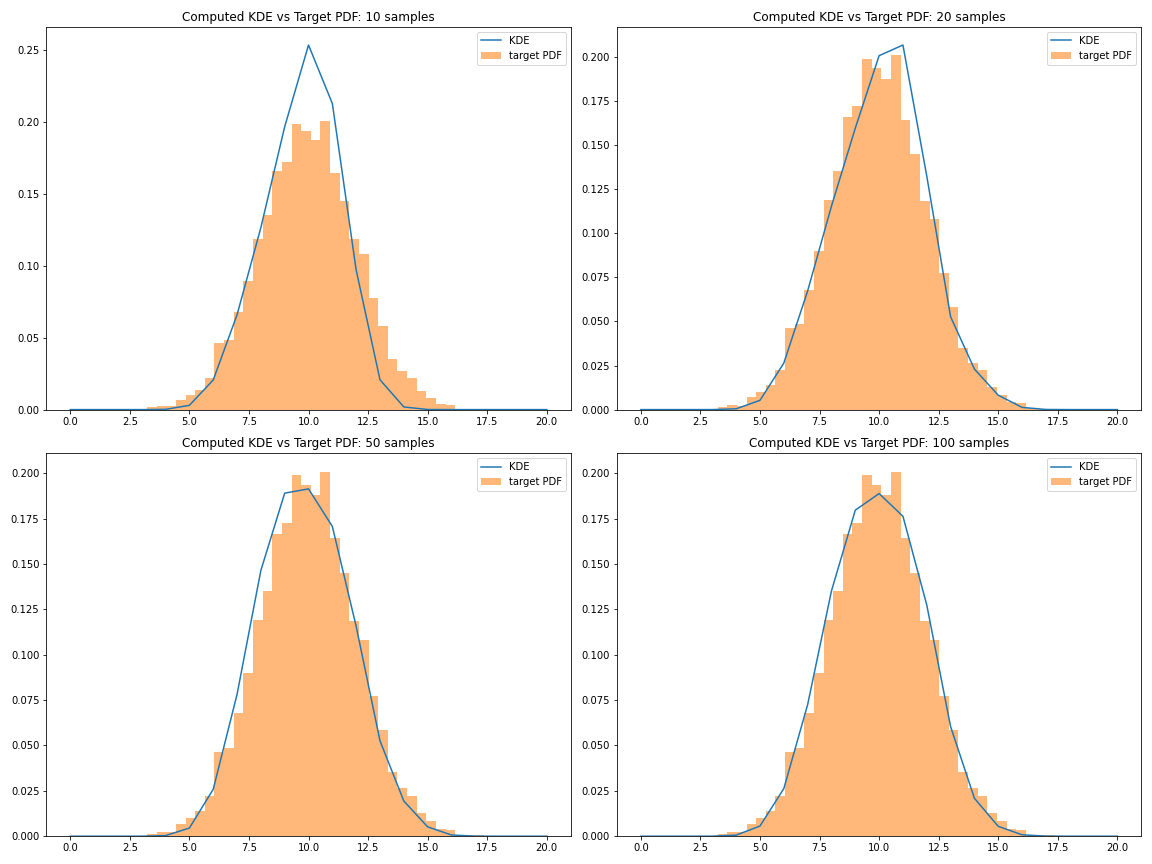
\includegraphics[width=0.82\textwidth]{13_team5_agentdesign/images/kde_plots.png}
    \caption{KDE simulation for a normal distribution for varying numbers of samples.}
    \label{fig:KDE_uniform}
\end{figure}

Another example of the efficacy of our KDE implementation is presented in Figure~\ref{fig:kde-exp}. Here, the distribution of disaster magnitudes - an exponential pdf - is estimated. The estimated PDF is remarkably close to the target, even with as few as 20 samples.

\begin{figure}[!htb]
    \centering
    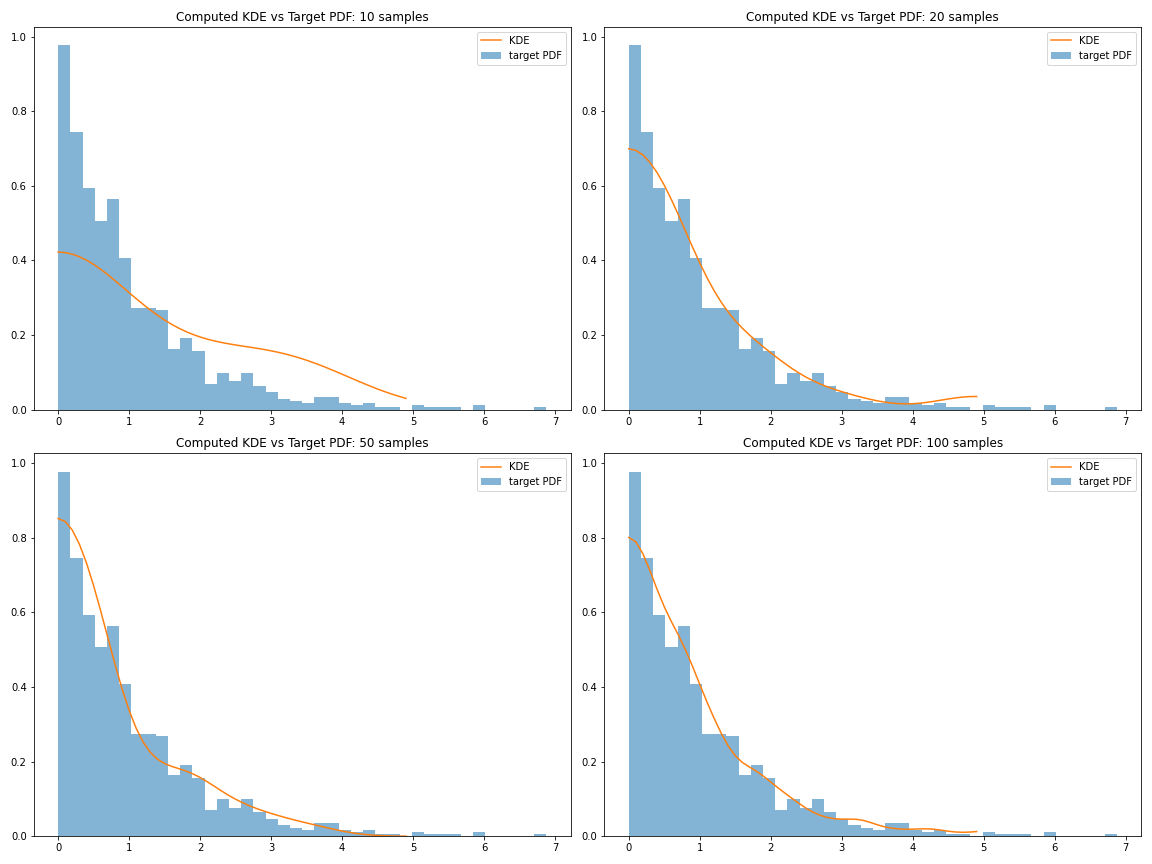
\includegraphics[width=0.82\textwidth]{13_team5_agentdesign/images/kde_plots_exp_deer_sizes.png}
    \caption{KDE of disaster magnitudes based on observed data against the true underlying exponential pdf for varying number of observed samples.}
    \label{fig:kde-exp}
\end{figure}

In our implementation, KDE was used to estimate the underlying distributions for each forecast variable of interest. These estimates evolve (become more accurate) with more data and so, our agent theoretically should become a more skilled forecaster with time.

\subsubsection{Confidence of forecasts}
Another important component of our agent's forecasts is its confidence. This is not only helpful in other decision making processes in our strategy (such as deciding how many resources to contribute to the Common Pool), but is also integral to our reputation amongst other agents. Clearly, if we're producing  inaccurate predictions with high confidence, other agents will quickly learn to no longer trust our forecasts and may begin to stop sharing their forecasting decisions. Therefore, confidence is used carefully and honestly in our implementation; with limited data or inadequate historical accuracy in our estimates, our prediction confidence will be low. As we receive more data and are able to verify the stability of our estimates, the associated prediction confidence increases gradually. 

Confidence for our agent's forecasts is computed based on the variance of observed data. Specifically, confidence $\kappa$ for a given variable $x$ is computed as follows in Equation~\ref{eq: Forecast Confidence}:

\begin{equation}
\kappa = \frac{\sigma_x}{\Delta_x} \quad \text{where} \quad \Delta_x = P_x^{(0.95)}-P_x^{(0.05)}
\label{eq: Forecast Confidence}
\end{equation}

In this definition, confidence is an effectively a notion of relative dispersion of the observed data. It is the ratio of the standard deviation of a variable $x$ and its range $\Delta_x$. Instead of the ordinary definition of range, $\Delta_x = P_x^{(0.95)}-P_x^{(0.05)}$ was used where $ P_x^{(n)}$ represents the $n^{\text{th}}$ percentile of $x$. This was decided to avoid the possibility of outliers obscuring $\kappa$. Evidently, if observed samples are densely packed around the mean value, $\sigma_x$ will be closer to $\Delta_x$ and confidence will be higher. The opposite is true for more dispersed observations.

\subsection{Collaboration}
The other important component of forecasting is incorporating forecasts from other teams. In each turn, we receive forecasts offered to us from other teams - a (possibly empty) subset of all teams. These collaborative forecasts are stored each turn. After each disaster occurs, our agent evaluates the \textit{forecast performance} of both itself and the other agents in the following manner:
\begin{enumerate}
    \item Analyse every forecast preceding the disaster and for each variable (magnitude, period etc), compute the squared error between the forecasted and actual values. 
    \item Compute the exponentially-weighted average of these errors for each variable. An exponential decay is chosen so as to weight more recent forecasts more. 
\end{enumerate}

Once these historically-aggregated forecasting errors are computed for all agents (including ours), we evaluate the forecasting skill of other agents relative to ours. For each agent (excluding our agent) and each forecast variable, compare the other agent's forecast error to ours in the following way in Equation~\ref{eq:Evaluate Forcasting Skills}:

\begin{equation}
\text{relative skill} = s := 1-\frac{\epsilon_i}{\epsilon_*},\quad i \in \mathcal{A}_i, \quad |s| \leq 1
\label{eq:Evaluate Forcasting Skills}
\end{equation}

where $\epsilon_i$ is the forecast error of of agent $i$ for a given variable, $\epsilon_*$ is our agent's error for this variable and $\mathcal{A}_i$ is the index set of all agents. This skill value $s$ can be interpreted as follows:

\begin{itemize}
    \item $s < 0$: other agent is less skillful than ours at forecasting a certain variable
    \item $s = 0$: other agent's skill is on par with that of our agent
    \item $s > 0$: other agent is more skillful than ours at forecasting a certain variable 
\end{itemize}

These skill values are directly used to update our perceived forecasting reputation (part of opinion) of other islands.

Our evaluation of the confidence of other agents' forecasts is performed in exactly the same manner as ours. Forecasts with unrealistic confidence values - either in the absolute sense or relative to the amount of data available - will be held in lower regard. The forecasting reputation (explored below) of the agents responsible for such forecasts would be adjusted accordingly. 

\subsubsection{Role of opinions in forecasting}
As described in Section~\ref{subsec: opinion-formation}, our agent's opinion formation is an important mechanism for choosing which agents to exchange forecasting information with. Specifically, the \texttt{forecastingReputation} variable stored in our agent's \texttt{opinionMap} represents its evaluation of the forecasting skill of each other agent based on historical data. Some examples of how the \texttt{forecastingReputation} of other agents is updated by our agent:
\begin{itemize}
    \item An agent's reputation value is decreased if they make a nonsensical prediction with over $50\%$ confidence before any disasters have occurred.
    \item Unfounded certainty is also punished: reputations are decreased if an agent makes a prediction with over $99\%$ confidence and our agent detects that predicted variables are stochastic.
    \item Reputations are updated after each disaster based on calculated \texttt{forecastingSkill} which, as described above, quantifies another agent's average forecasting accuracy relative to ours. 
\end{itemize}

These reputation scores allow our agent to decide which agents' forecasting information to trust. Similarly, opinions allow our agent to choose which agents to share our \textit{precious} forecasting information with - if we simply share it indiscriminately, other agents may be less compelled to share their data as they would not lose in anything in not doing so. 

\section{Roles}
\subsection{President}
When our agent gets voted to be the the President, the following steps elaborate the strategy the President is going to take for each action point.
The President's role is to evaluate and allocate the common pool request resources. In order to evaluate a common pool request, the President assesses the size of the request and the current size of the common pool.The resource allocation has been divided into three possible scenarios: 
    \begin{itemize}
        \item If the request total is smaller than $80\%$ of the size of the common pool, then the President allocates all the requests.
        \item If the request total is between $80\%$ and the common pools current value, then the President divides the requests by two and then allocates them.
        \item If the request total is higher than the common pool size, then the President returns a fraction of those resources to the islands, keeping the common pool dynamics in order.
    \end{itemize}

Another commitment of the President is to set taxation amount to individual islands. Tax is necessary for IIGO roles and procedures to work. The President aims to set a fair tax amount to individuals proportional to their wealth. However, if an island chooses not report their wealth, a flat tax rate will be applied, which is high enough to encourage agents to be transparent about their resources. 

Furthermore, the islands will propose different sets of rules to alter the game specification, and the President selects one of the proposed rules to vote on.    
The President must also pay the Speaker its salary, for the Speaker to complete its tasks. In addition, the speakers salary is proportional to our agent's wealth. 
    \begin{itemize}
        \item When our agent is in \texttt{jeffBezos} tier, then, the Speaker salary is payed in full.
        \item When our agent has \texttt{middleClass} wealth tier, then only $80\%$ of the speakers salary is payed.
        \item When our agent is poor, which mean it is in \texttt{imperialStudent} wealth state, then only half of the speakers salary is paid.
    \end{itemize}

This strategy of paying the Speaker emphasizes the importance of preserving the Common Pool to the islands in difficult times. Since the agent has no way to look at others' wealth, it makes a rough estimation based on its own wealth. And since the common pool allocation strategy has no bias to any particular agent, the common pool is preserved for the well-being of agent in the difficult time. 

The President also has the task to decide the next Speaker. The President can manipulated the Speaker election and assigns the next Speaker based on our opinion of each team. The reason this strategy was implemented is because the agent's opinion is formed mostly based how much other agents try to help fellow agents. And it is an important characteristic that an important role should have.    

Moreover, the President sets the tax amount every turn, the tax rate is designed to be proportional to the islands resources in order to provide fair division of resources. However, if an island does not report their resources, then a strict tax rate is applied, which will essentially influence the islands to share the value of their resources with other islands. Additionally, the President is responsible to monitor the Judge's behaviour and hold the Speaker's election. 

\subsection{Speaker and Judge}
When our agent gets voted to become the Speaker or Judge, the following steps elaborate the strategy the agent is going to take for each action point.
The Judge has the privilege to pardon other islands. The Judge pardons agents who are highly regarded based on opinion scores. Similar to President's strategy, the agent pays the other role in the following way  to ensure the common pool's main focus is agents in difficult times. 

    \begin{itemize}
        \item When our agent is in \texttt{jeffBezos} tier, then the other role's salary is paid in full.
        \item When our agent has \texttt{middleClass} wealth tier, then only $80\%$ of salary is paid.
        \item When our agent is poor, which mean it is in \texttt{imperialStudent} wealth state, then only $50\%$ of the salary is paid.
    \end{itemize}
    
Furthermore, the Speaker and Judge hold elections for the other roles, a real winner will be voted on by the islands, but then our agent will announce the next Judge based on our opinions for aforementioned reasons.
    \begin{itemize}
        \item If our agent has bad opinion towards the real winner, which means opinion score is inferior to $0$, then our agent will choose another agent with highest opinion score to become the next Judge.
        \item if the real winner is on our agent's good side (a friend, score $> 0$), then he will be announced as the new role.
    \end{itemize}

\subsection{Voting for IIGO Roles}
Voting for IIGO roles are done based on our agent's current opinion on other agents. Our agent will always put itself on top of the vote and fill in other contestant from the candidate list based on opinion score from highest to lowest. This is a fair strategy to determine the IIGO roles since the agent's opinion is influenced by the interaction and devotion of other agents to the community. 

\subsection{Future work}
Currently, the agent only have one persona when acting as an official role. The personality of the role could be driven by its current wealth. Say if the agent is in \texttt{imperialStudent} state, it may try to find as much resources as possible, no matter how corrupted the process may be. The different personalities will add more dynamic to the simulation and it would be interesting to see how the agent would thrive or decline with different scenarios. 
\section{Simulation}

This section details the dynamics observed during the simulation of our agent's behaviour the other islands in the Archipelago. Once all agent implementations were finalised, simulations were performed using \textit{baseline} parameters. There is an extensive list of parameters that can be changed with no sensible initial values for many parameters, thus these baseline values had to be determined empirically. The environment is built on a variety of probabilistic models that introduce a lot of variance to the simulations. With this in mind, multiple simulations were run to allow us to evaluate our agent's behaviour in a broader sense.

By adjusting a single environmental parameter whilst fixing the rest we could capture the effect of a single parameter on our agent as well as the other agents. All tests were run twice so that extreme scenarios could be mitigated to some extent. If two consecutive tests returned similar results, these could be included in the overview\footnote{behaviours or results with sufficiently low variance to characterise with a general value or outcome} results.


\subsubsection{Foraging}

The objective was to observe the effect of altering foraging parameters on our agent's behaviour. Performance is quantified by the foraging efficiency of our agent, which is the ratio of output utility to resources invested. The selected parameters were varied around the baseline values and were then compared to baseline performance\footnote{performance using the relevant metric but with baseline parameters}

We first focus on deer hunting, using  \texttt{input proportional} and \texttt{equally distributed} return of the resources. The results are displayed in Table~\ref{fig:Foraging Deer Hunting Parameter Simulation Results}.

\begin{figure} [!htb]
    \centering
    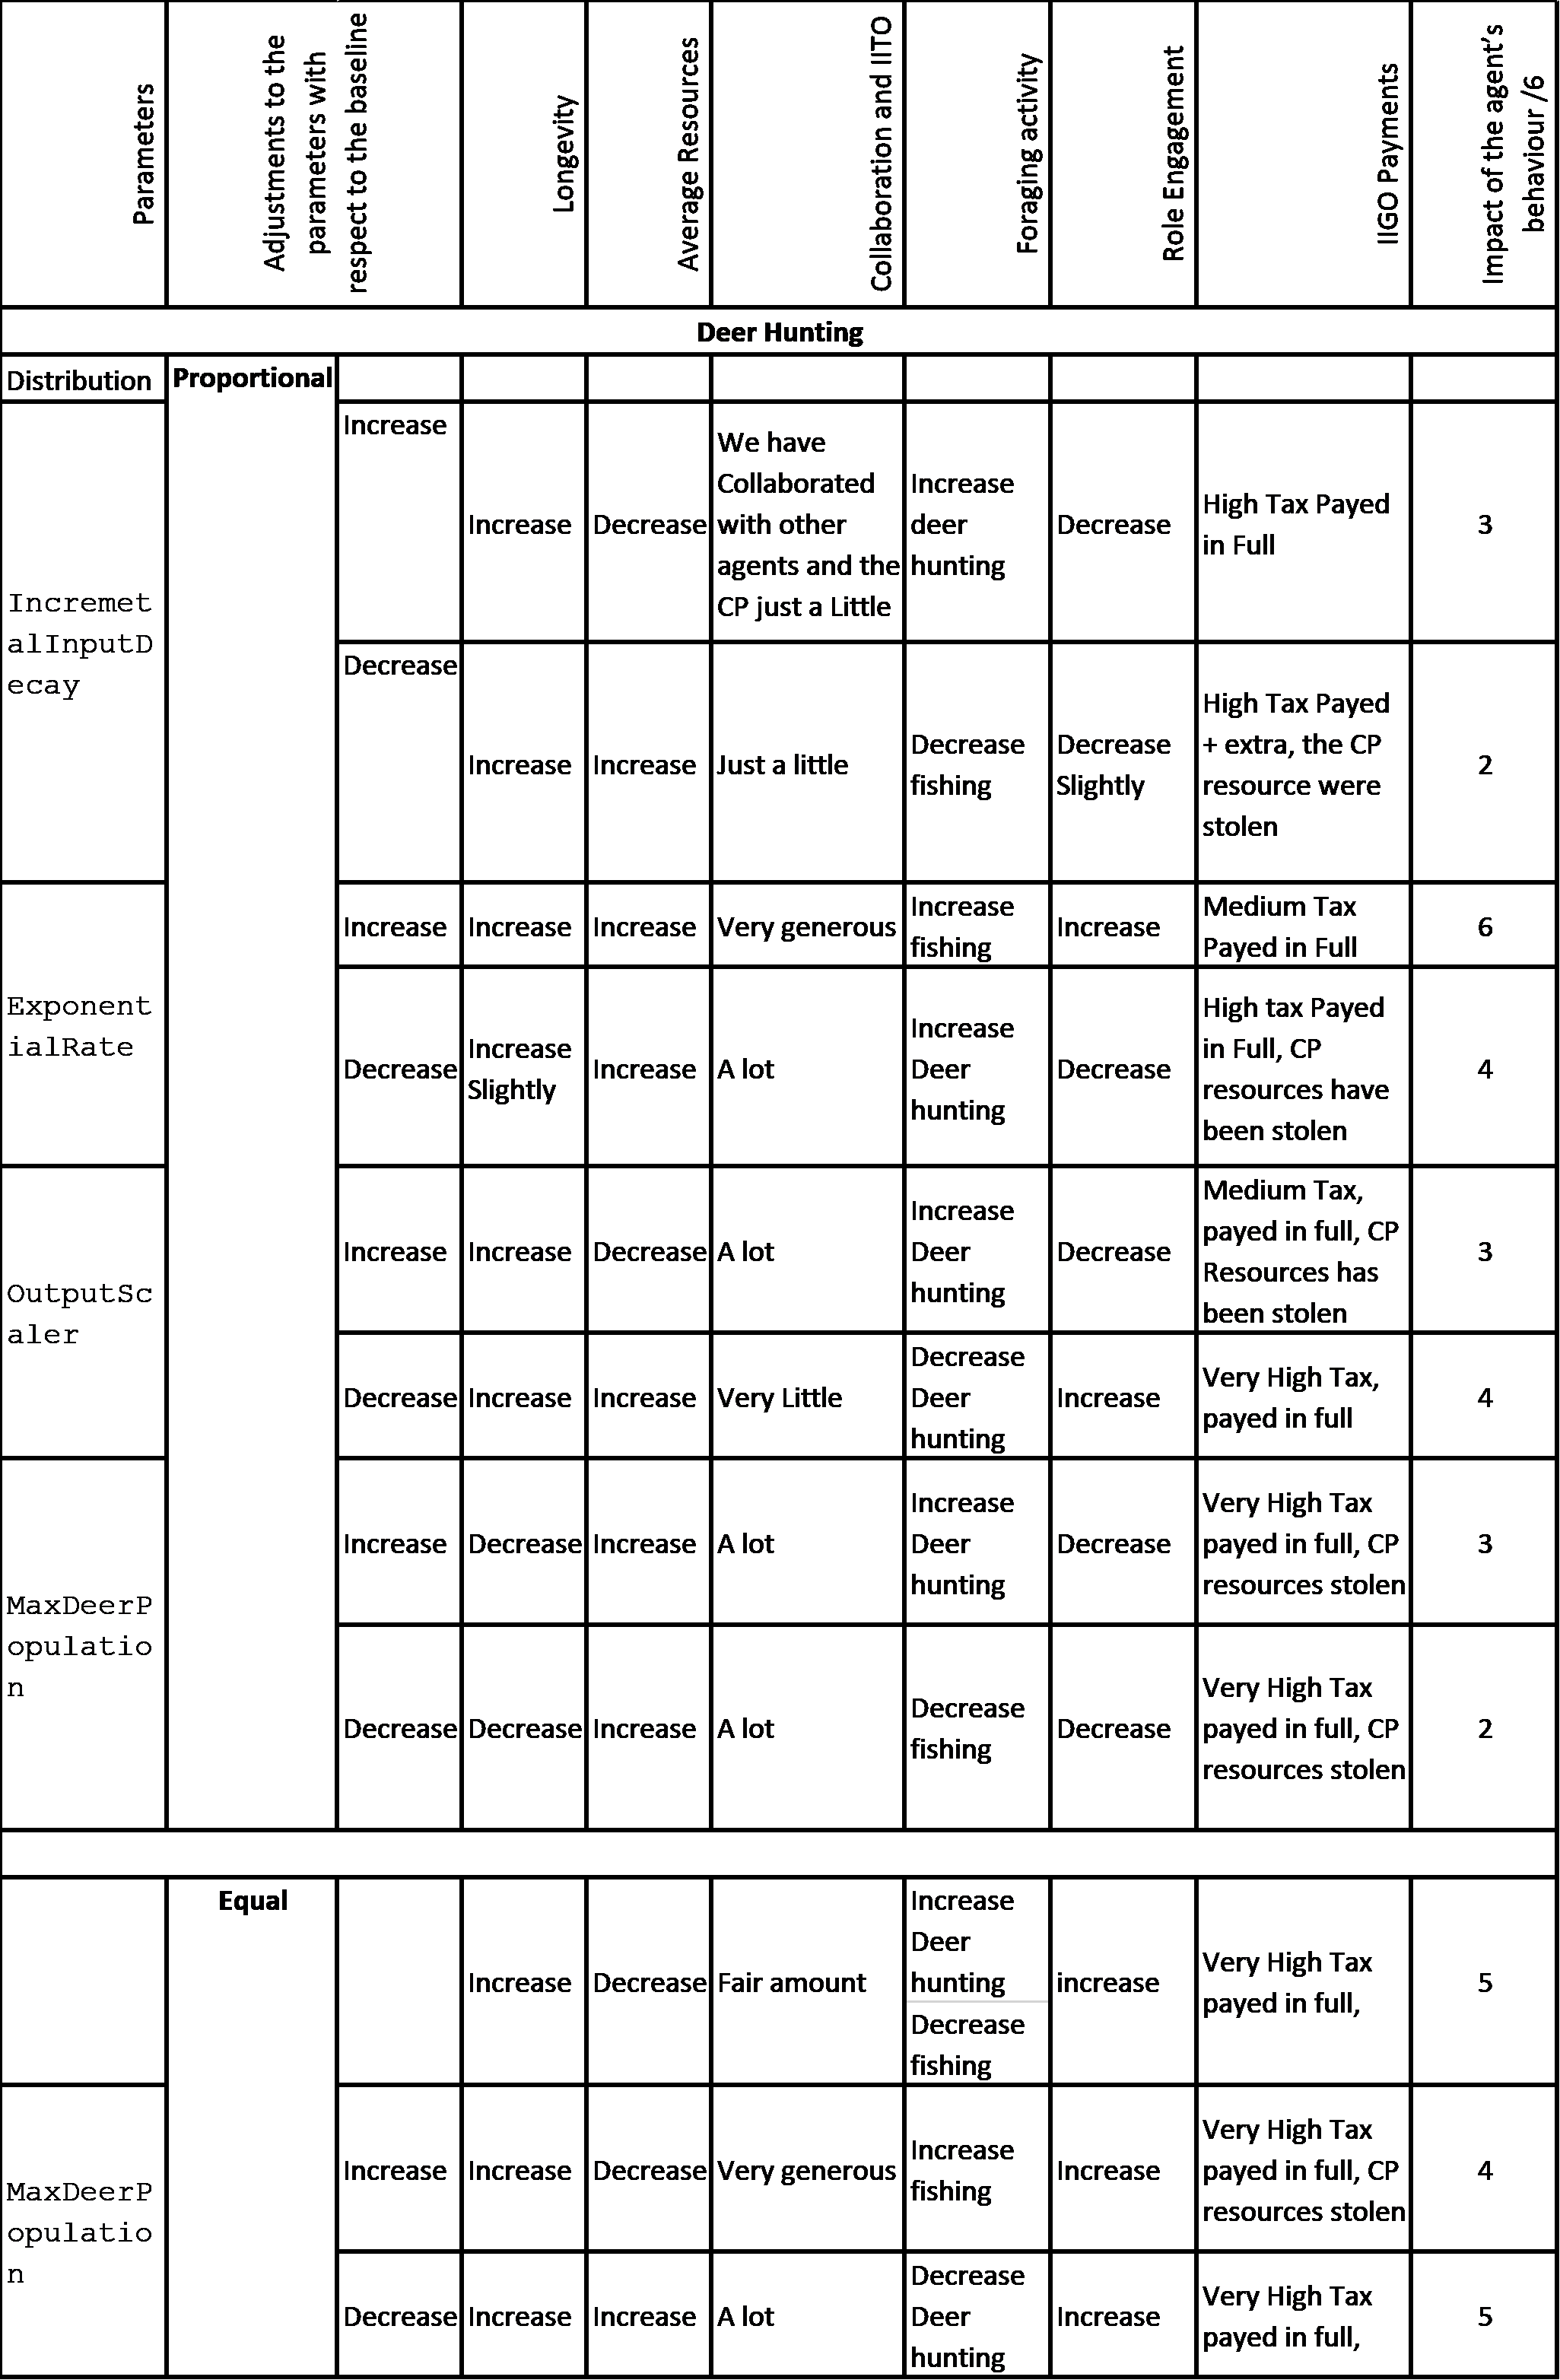
\includegraphics[width=1\textwidth]{13_team5_agentdesign/images/Foarging Simulation Deer Hunting.png}
    \caption{Foraging Deer Hunting Parameter Simulation Results}
    \label{fig:Foraging Deer Hunting Parameter Simulation Results}
\end{figure}

Next we changed the deer \texttt{OutputScaler} parameter. Once increased, we notice Figure~\ref{fig:Agent Resources Inversely correlated with the common Pool} shows that our agent is inversely correlated to the common pool resources. Therefore, the common pool resources decrease while our agent's resources increase, and vice versa.

\begin{figure}[!htb]
    \centering
    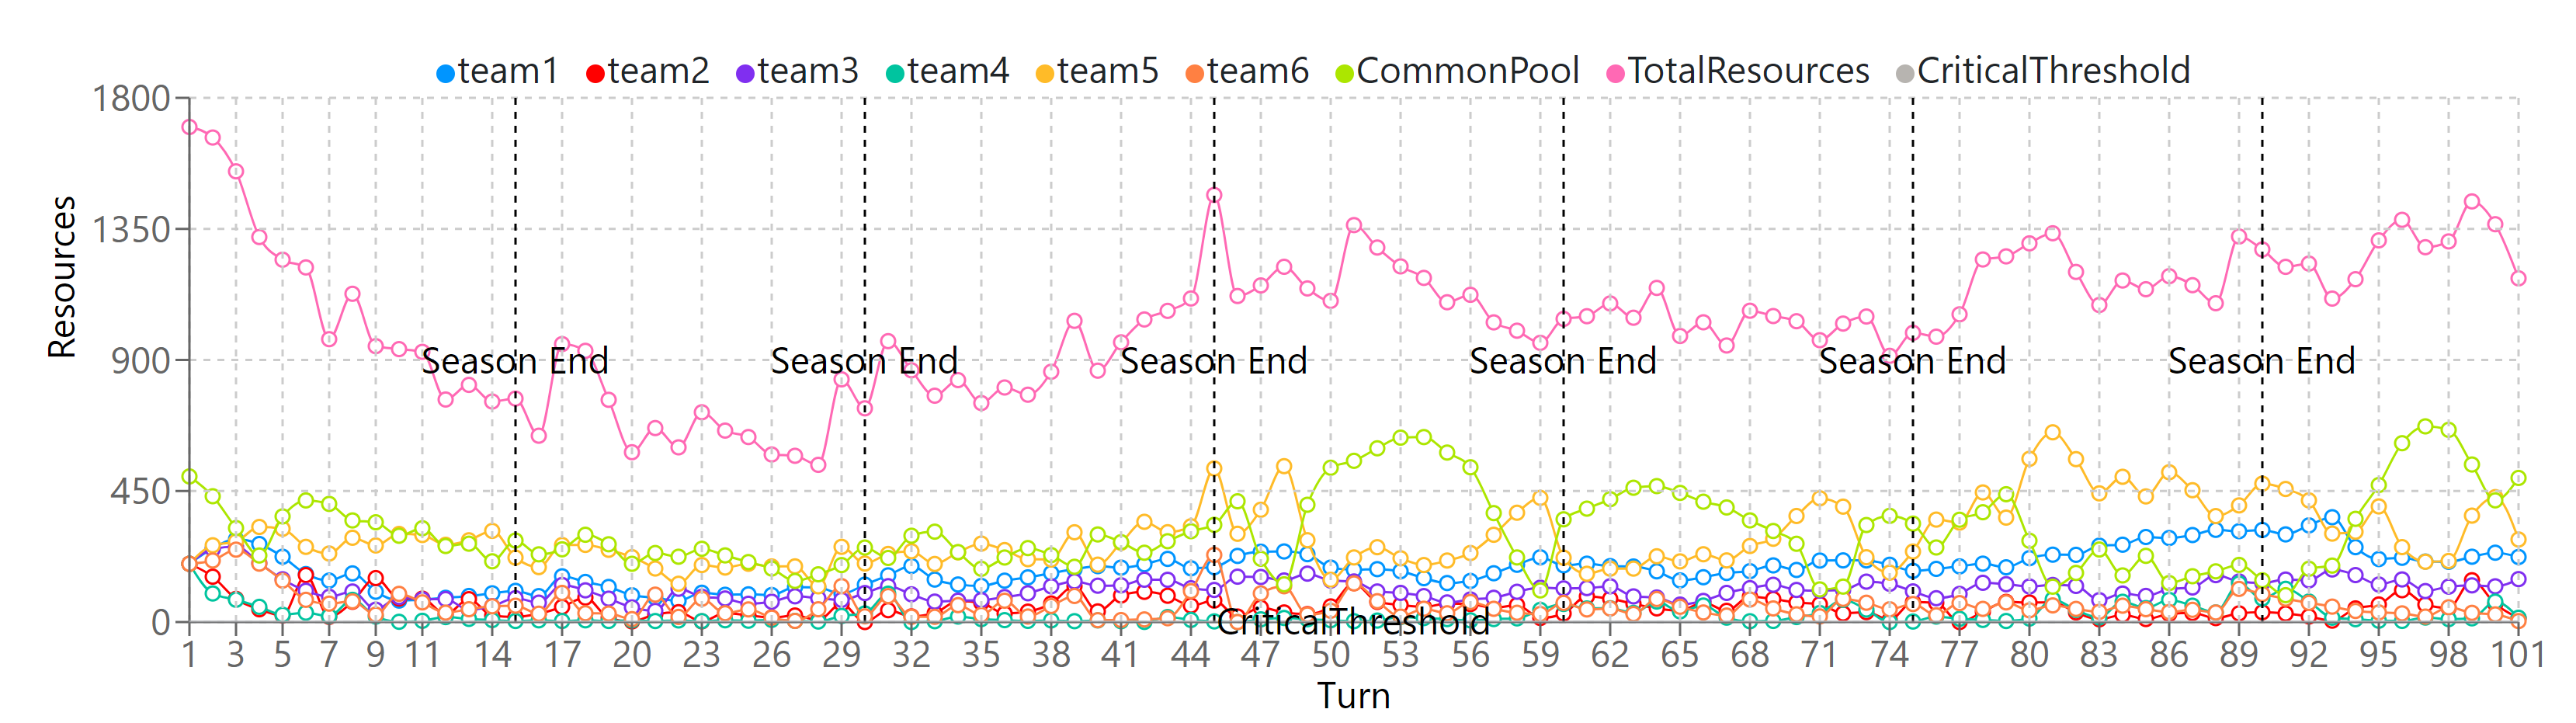
\includegraphics[width=0.9\textwidth]{13_team5_agentdesign/images/Agent Resources Inveserly correlated.png}
    \caption{Agent Resources Inversely correlated with the common Pool}
    \label{fig:Agent Resources Inversely correlated with the common Pool}
\end{figure}


We then altered the \texttt{MaxDeerPopulation} parameter for deer hunting with a input proportional\footnote{collective utility from the hunt is distributed proportionally to participants' contributions} resource return strategy. Our agent tend to live longer than in the baseline. However, with lower average resources.

Furthermore, the same parameter (\texttt{MaxDeerPopulation}) was tested for an equal utility distribution strategy. In this case, the agent's performs improved massively compared to the previously tested proportional distribution method: The agent became more generous with gifting and tended to survive considerably longer. Furthermore, the agent held more IIGO roles, which helped it accumulate more resources, allowing it to invest more into foraging.

When comparing the two methods of distribution, Figure~\ref{fig:Foraging Simulation MaxDeerpop_Prob} shows that the deer hunt is stable for both methods. However, For the equal distribution strategy as illustrated in Figure~\ref{fig:Foraging Simulation MaxDeerpop_Equal}, foraging activity increased substantially, as well as the foraging efficiency. 

\begin{figure}[!htb]
    \centering
    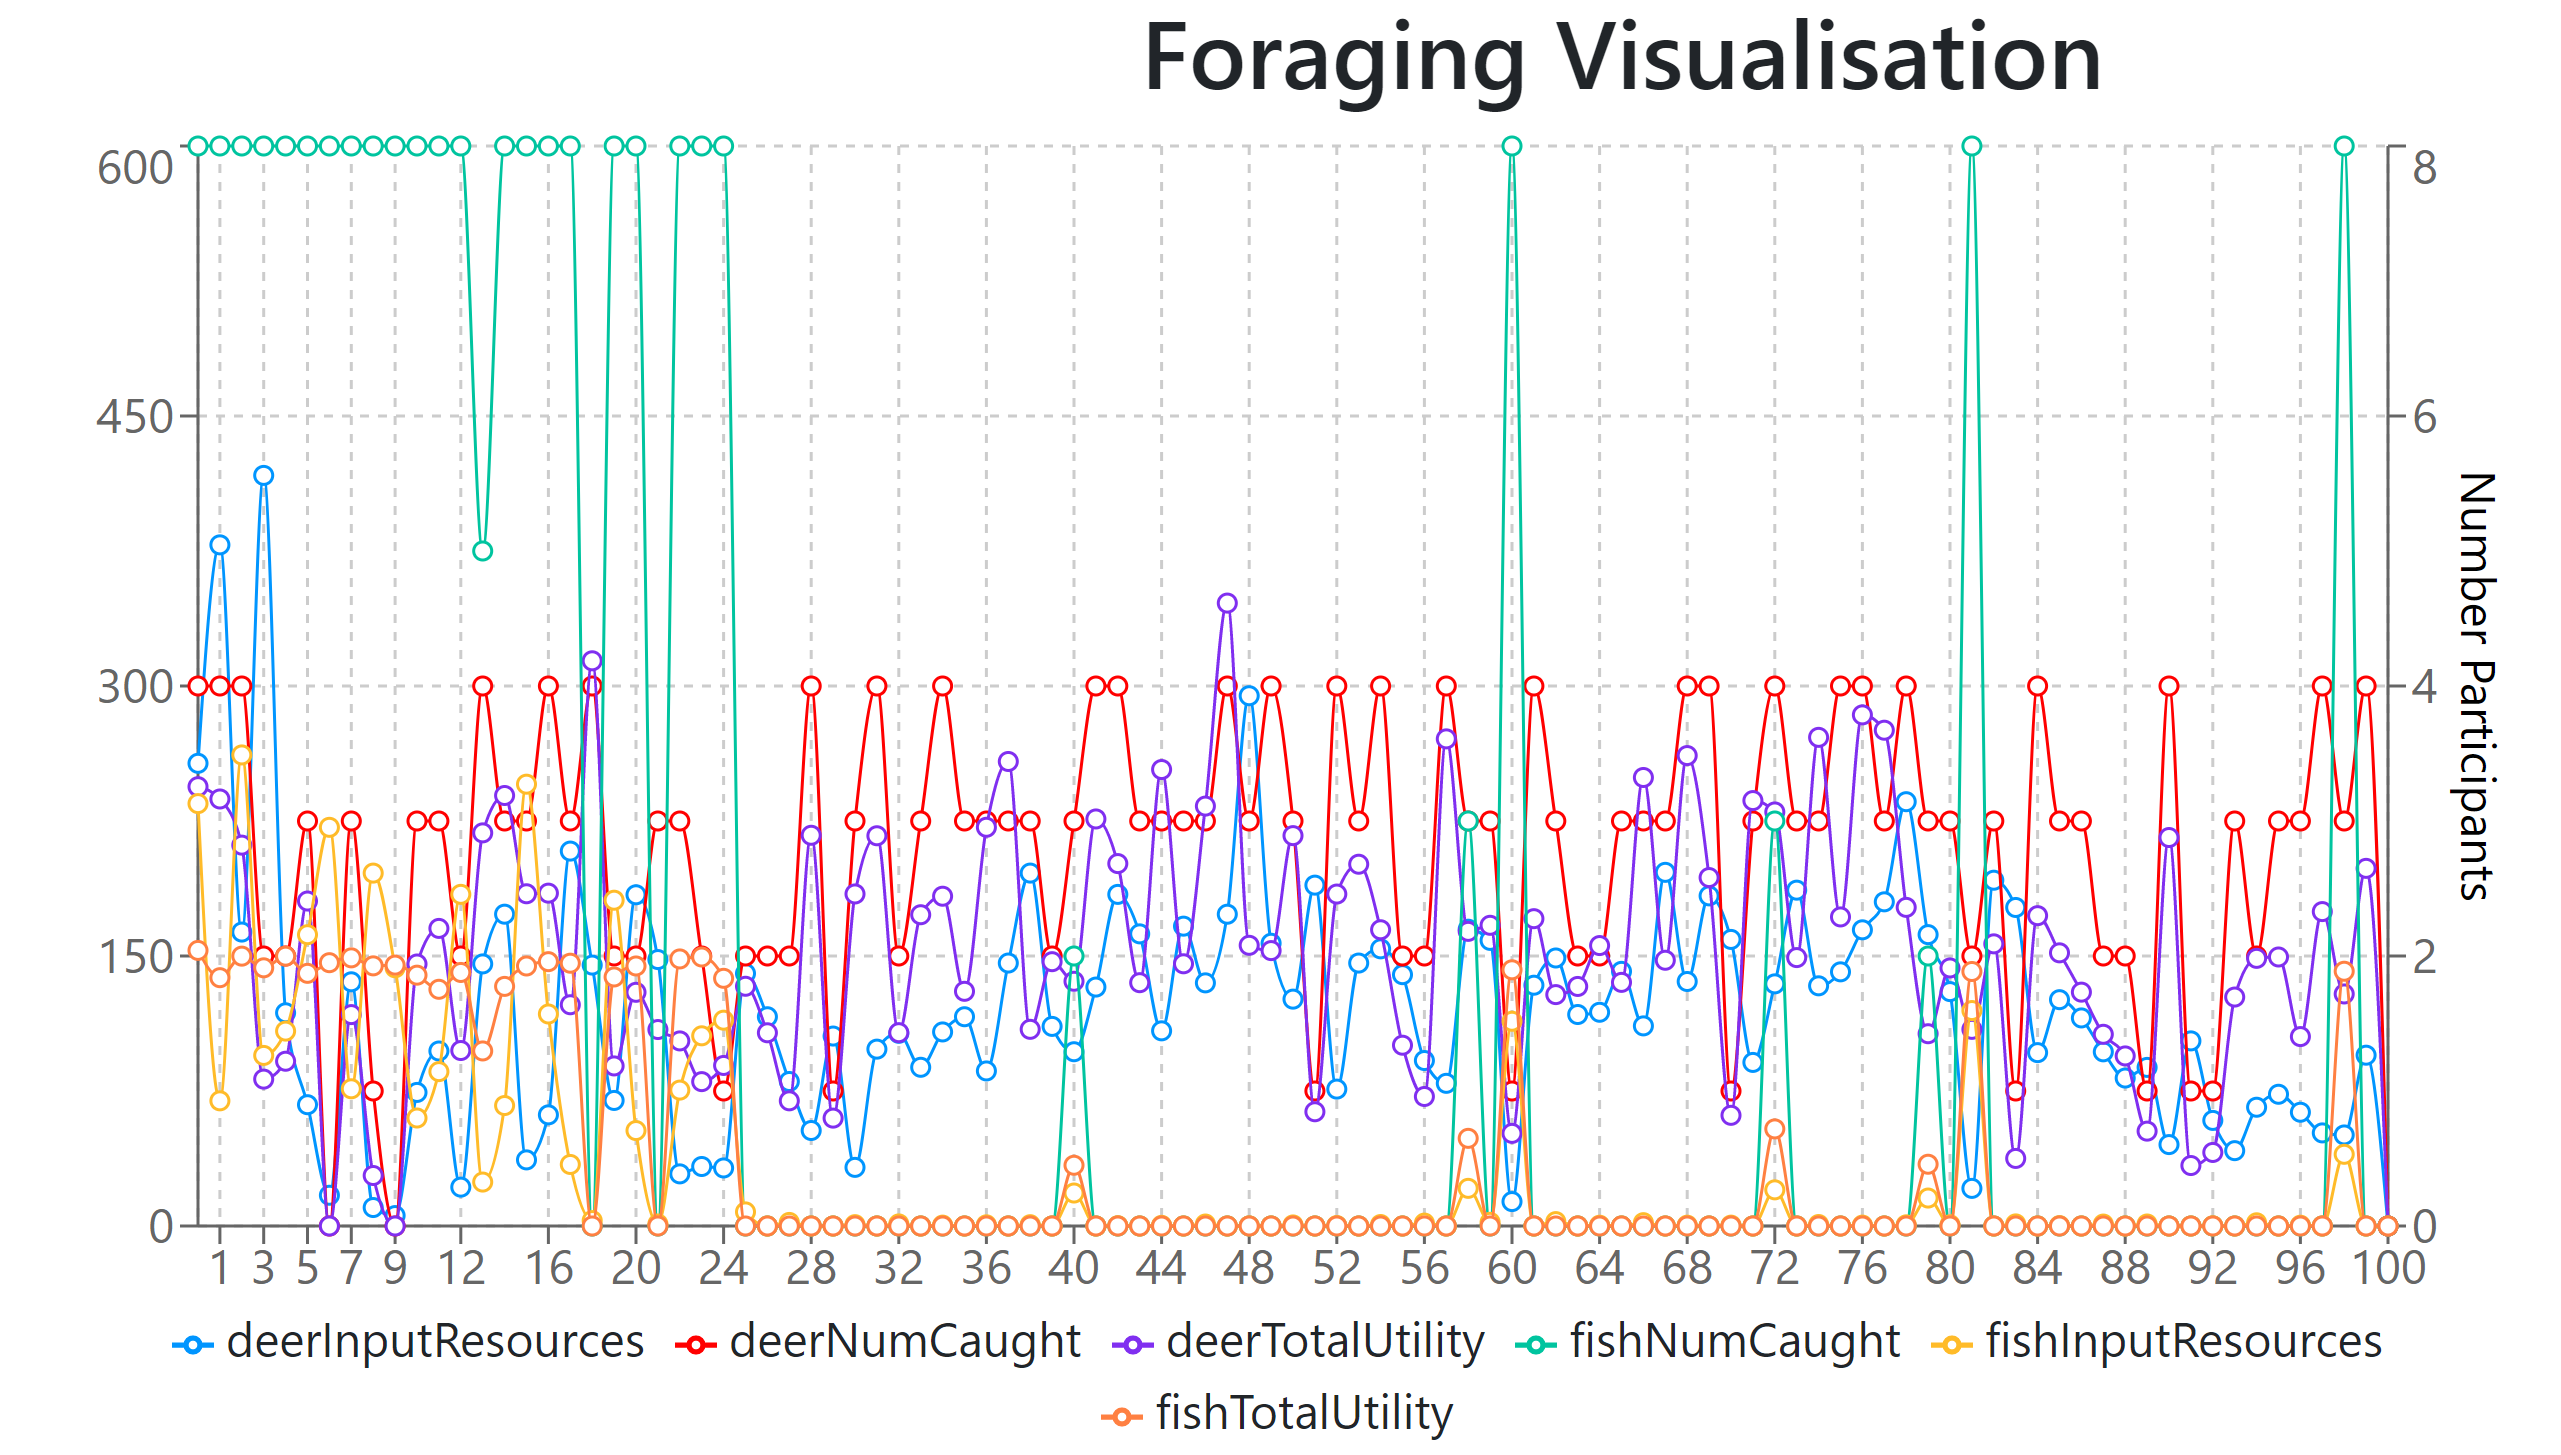
\includegraphics[width=0.8\textwidth]{13_team5_agentdesign/images/Foraging Simulation MaxDeerpop_Prob.PNG}
    \caption{Foraging Visualisation for a proportional distribution}
    \label{fig:Foraging Simulation MaxDeerpop_Prob}
\end{figure}

\begin{figure}[!htb]
    \centering
    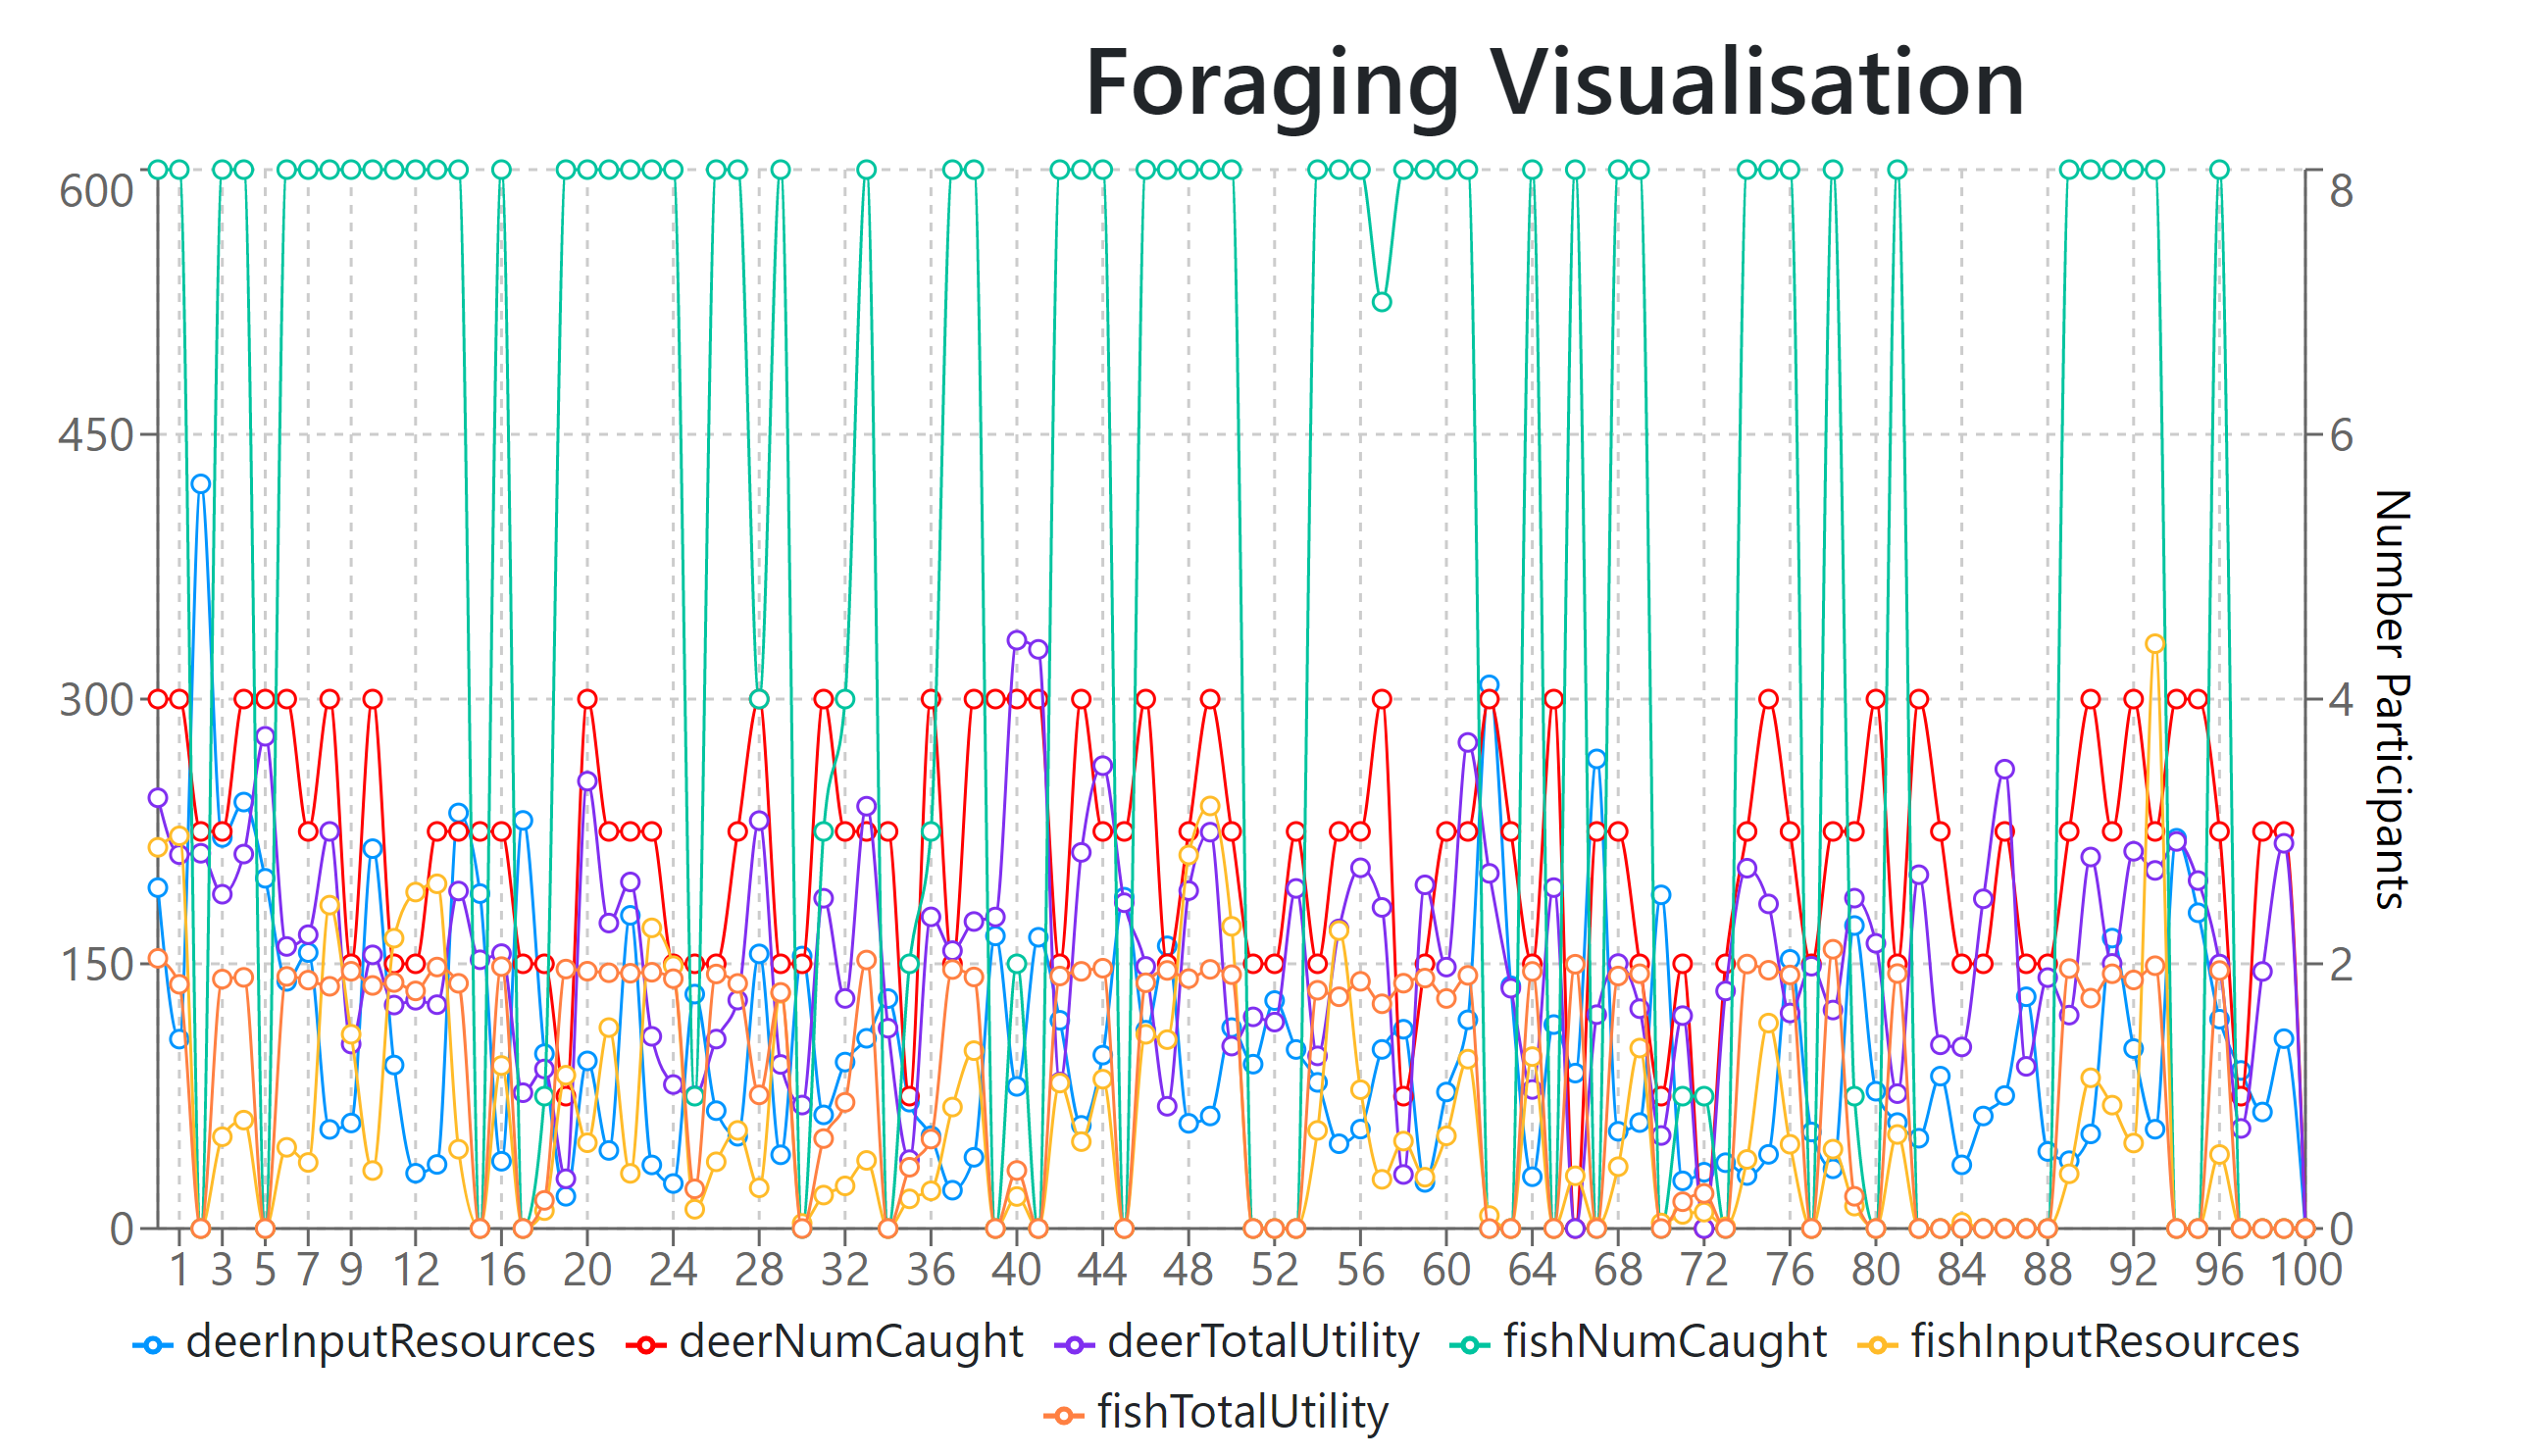
\includegraphics[width=0.8\textwidth]{13_team5_agentdesign/images/Foraging Simulation MaxDeerpop_Equal.PNG}
    \caption{Foraging Visualisation for an Equal distribution}
    \label{fig:Foraging Simulation MaxDeerpop_Equal}
\end{figure}

When the maximum deer population parameter in the game increases, the agent attempts to hunt as many deer as possible in a turn (as shown in Figure~\ref{fig:Foraging Simulation MaxDeerpop_Equal}, illustrated in the red line which is limited to a maximum of four deer that can be caught per turn). Whereas, when that parameter decreases, the agent reduces the amount of deer hunting and focuses more on fishing (Figure~\ref{fig:Foraging Simulation MaxDeerpop_Equal_decrease} - the green line represents the number of fish caught and the red line, the number of deer caught)

\begin{figure}[!htb]
    \centering
    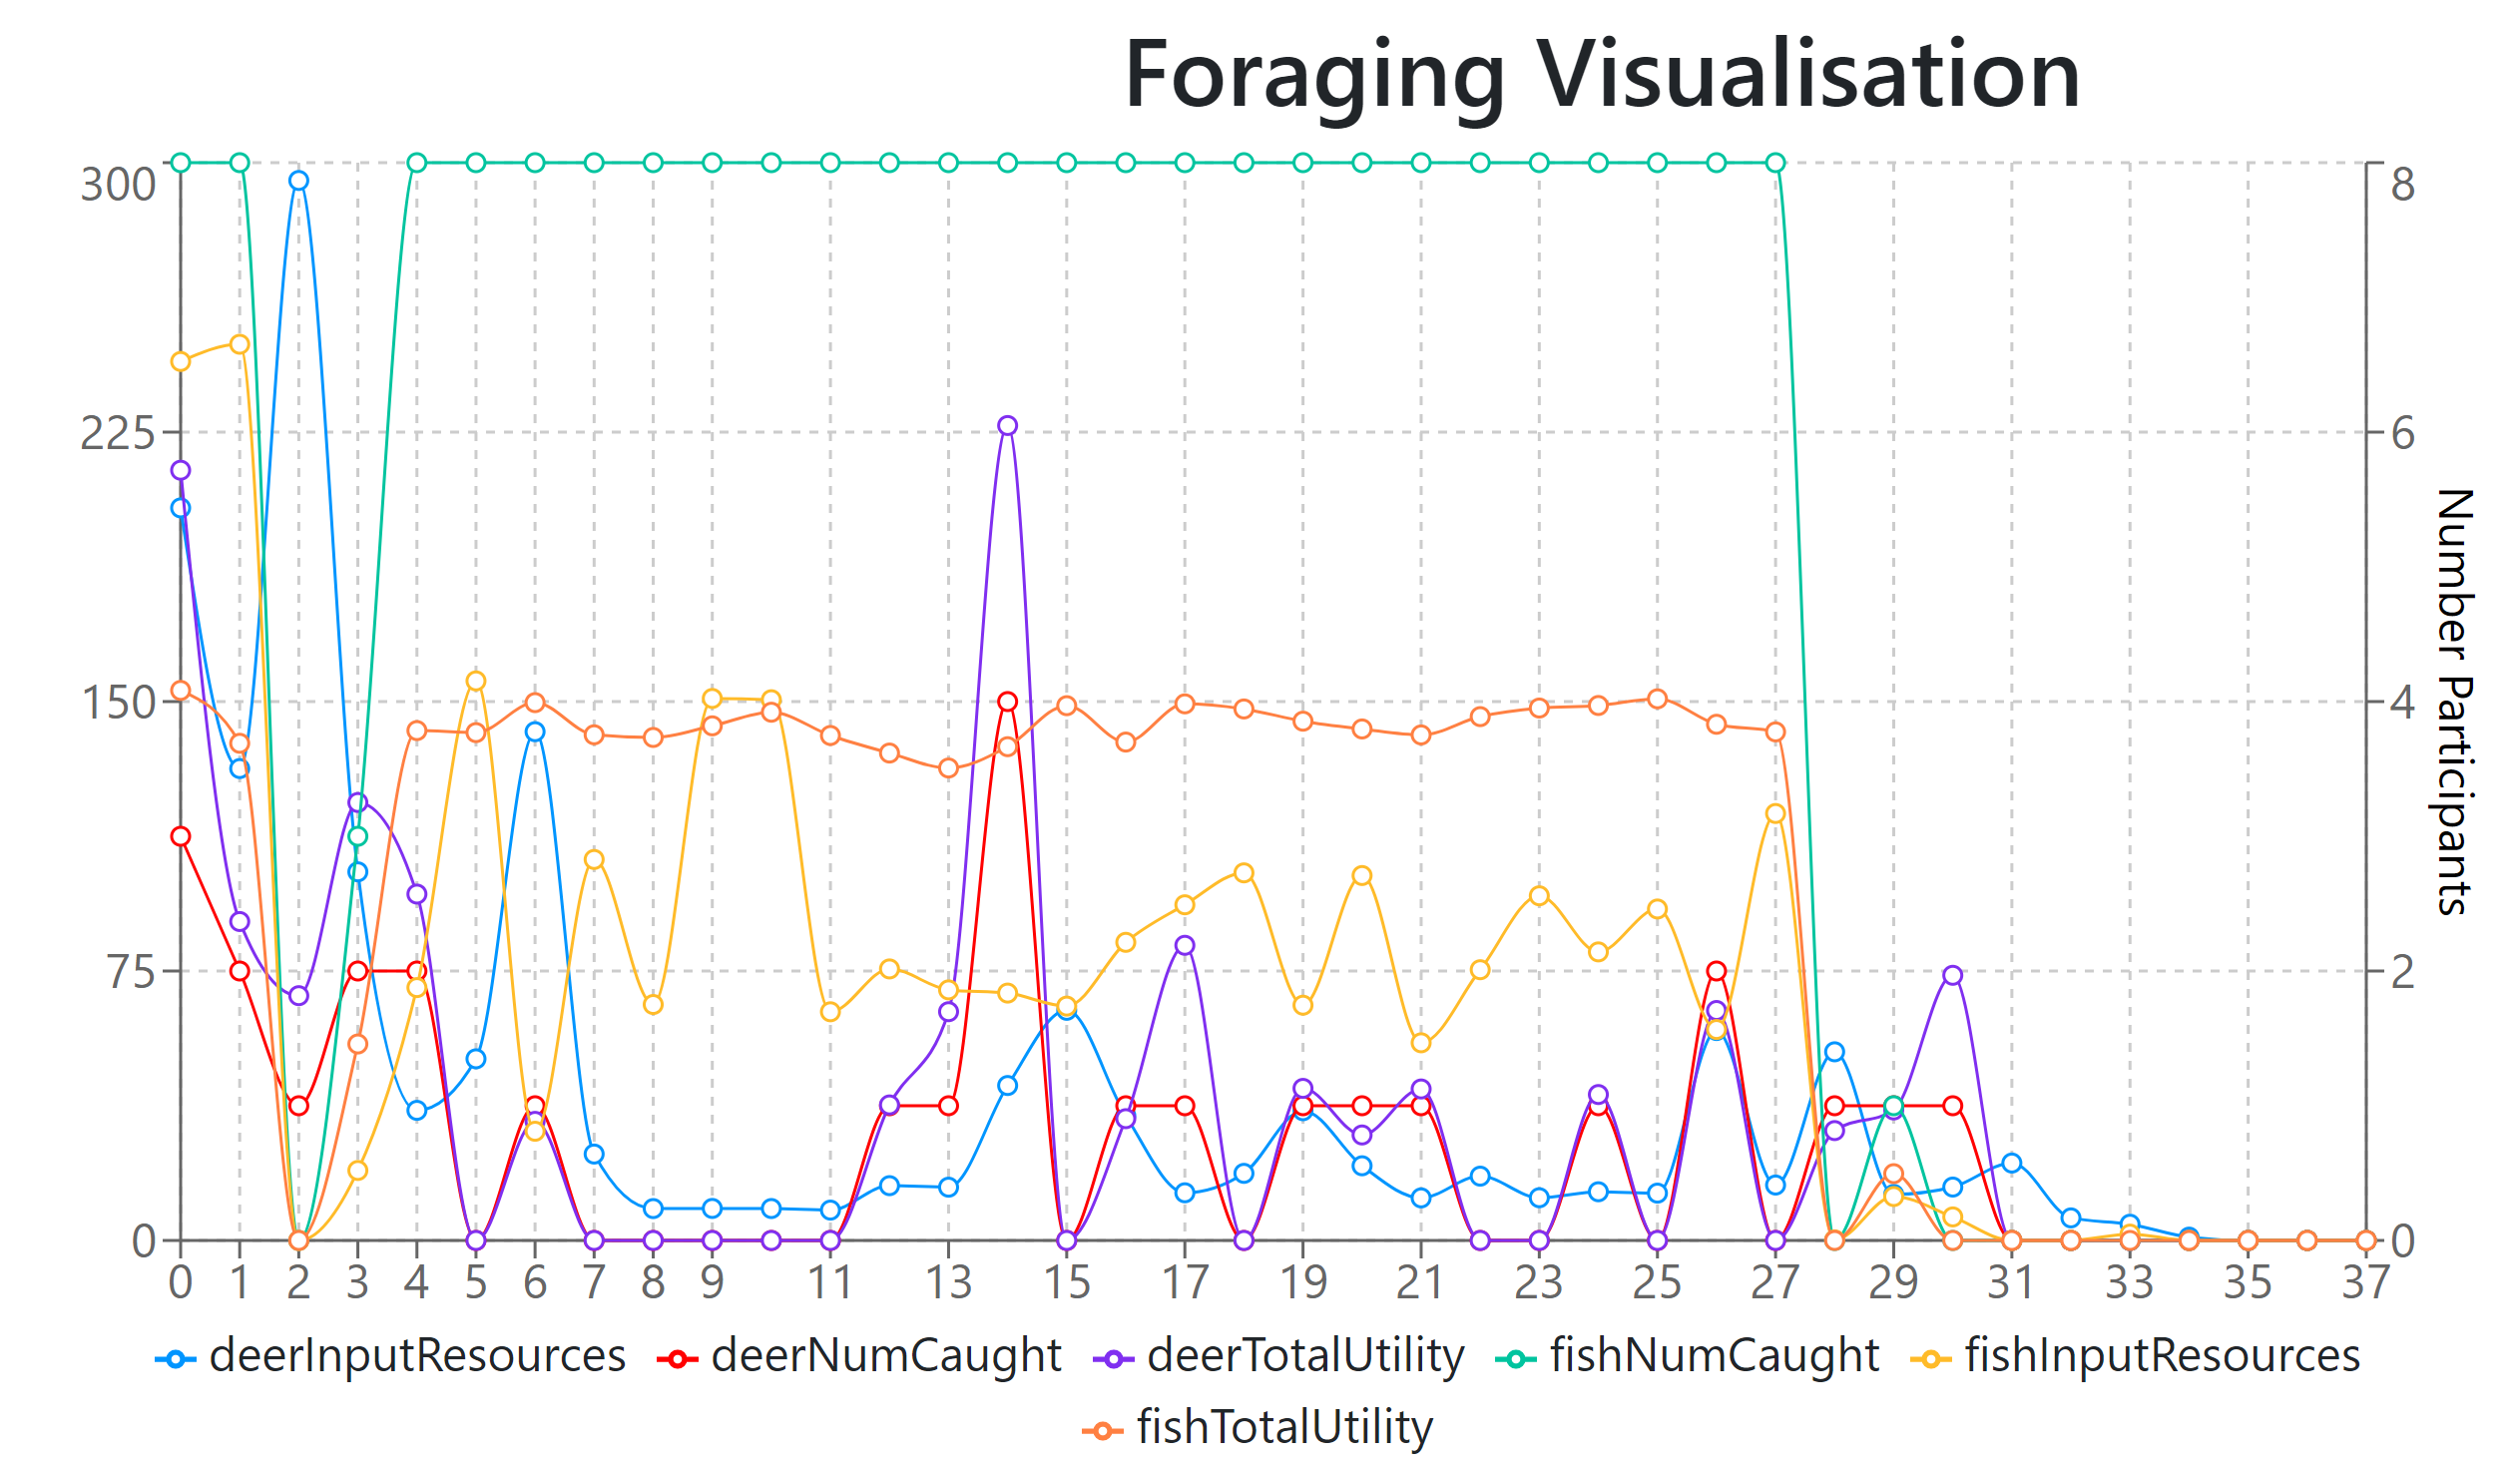
\includegraphics[width=0.8\textwidth]{13_team5_agentdesign/images/Foraging Simulation MaxDeerpop_Equal_decrease.PNG}
    \caption{Foraging Visualisation for an Equal distribution with a small Maximum Deer population Value}
    \label{fig:Foraging Simulation MaxDeerpop_Equal_decrease}
\end{figure}

It was spotted that our agent's tendency to over-invest into deer hunting. While the reward is high, the agent is over investing where lower contributions could lead to similar results.

Moreover, Fishing parameters have been altered to evaluate the behaviour and foraging efficiency of our agent. The simulated results are in Table~\ref{fig:Foraging Fishing parameters Simulation Results}.

\begin{figure}[!htb]
    \centering
    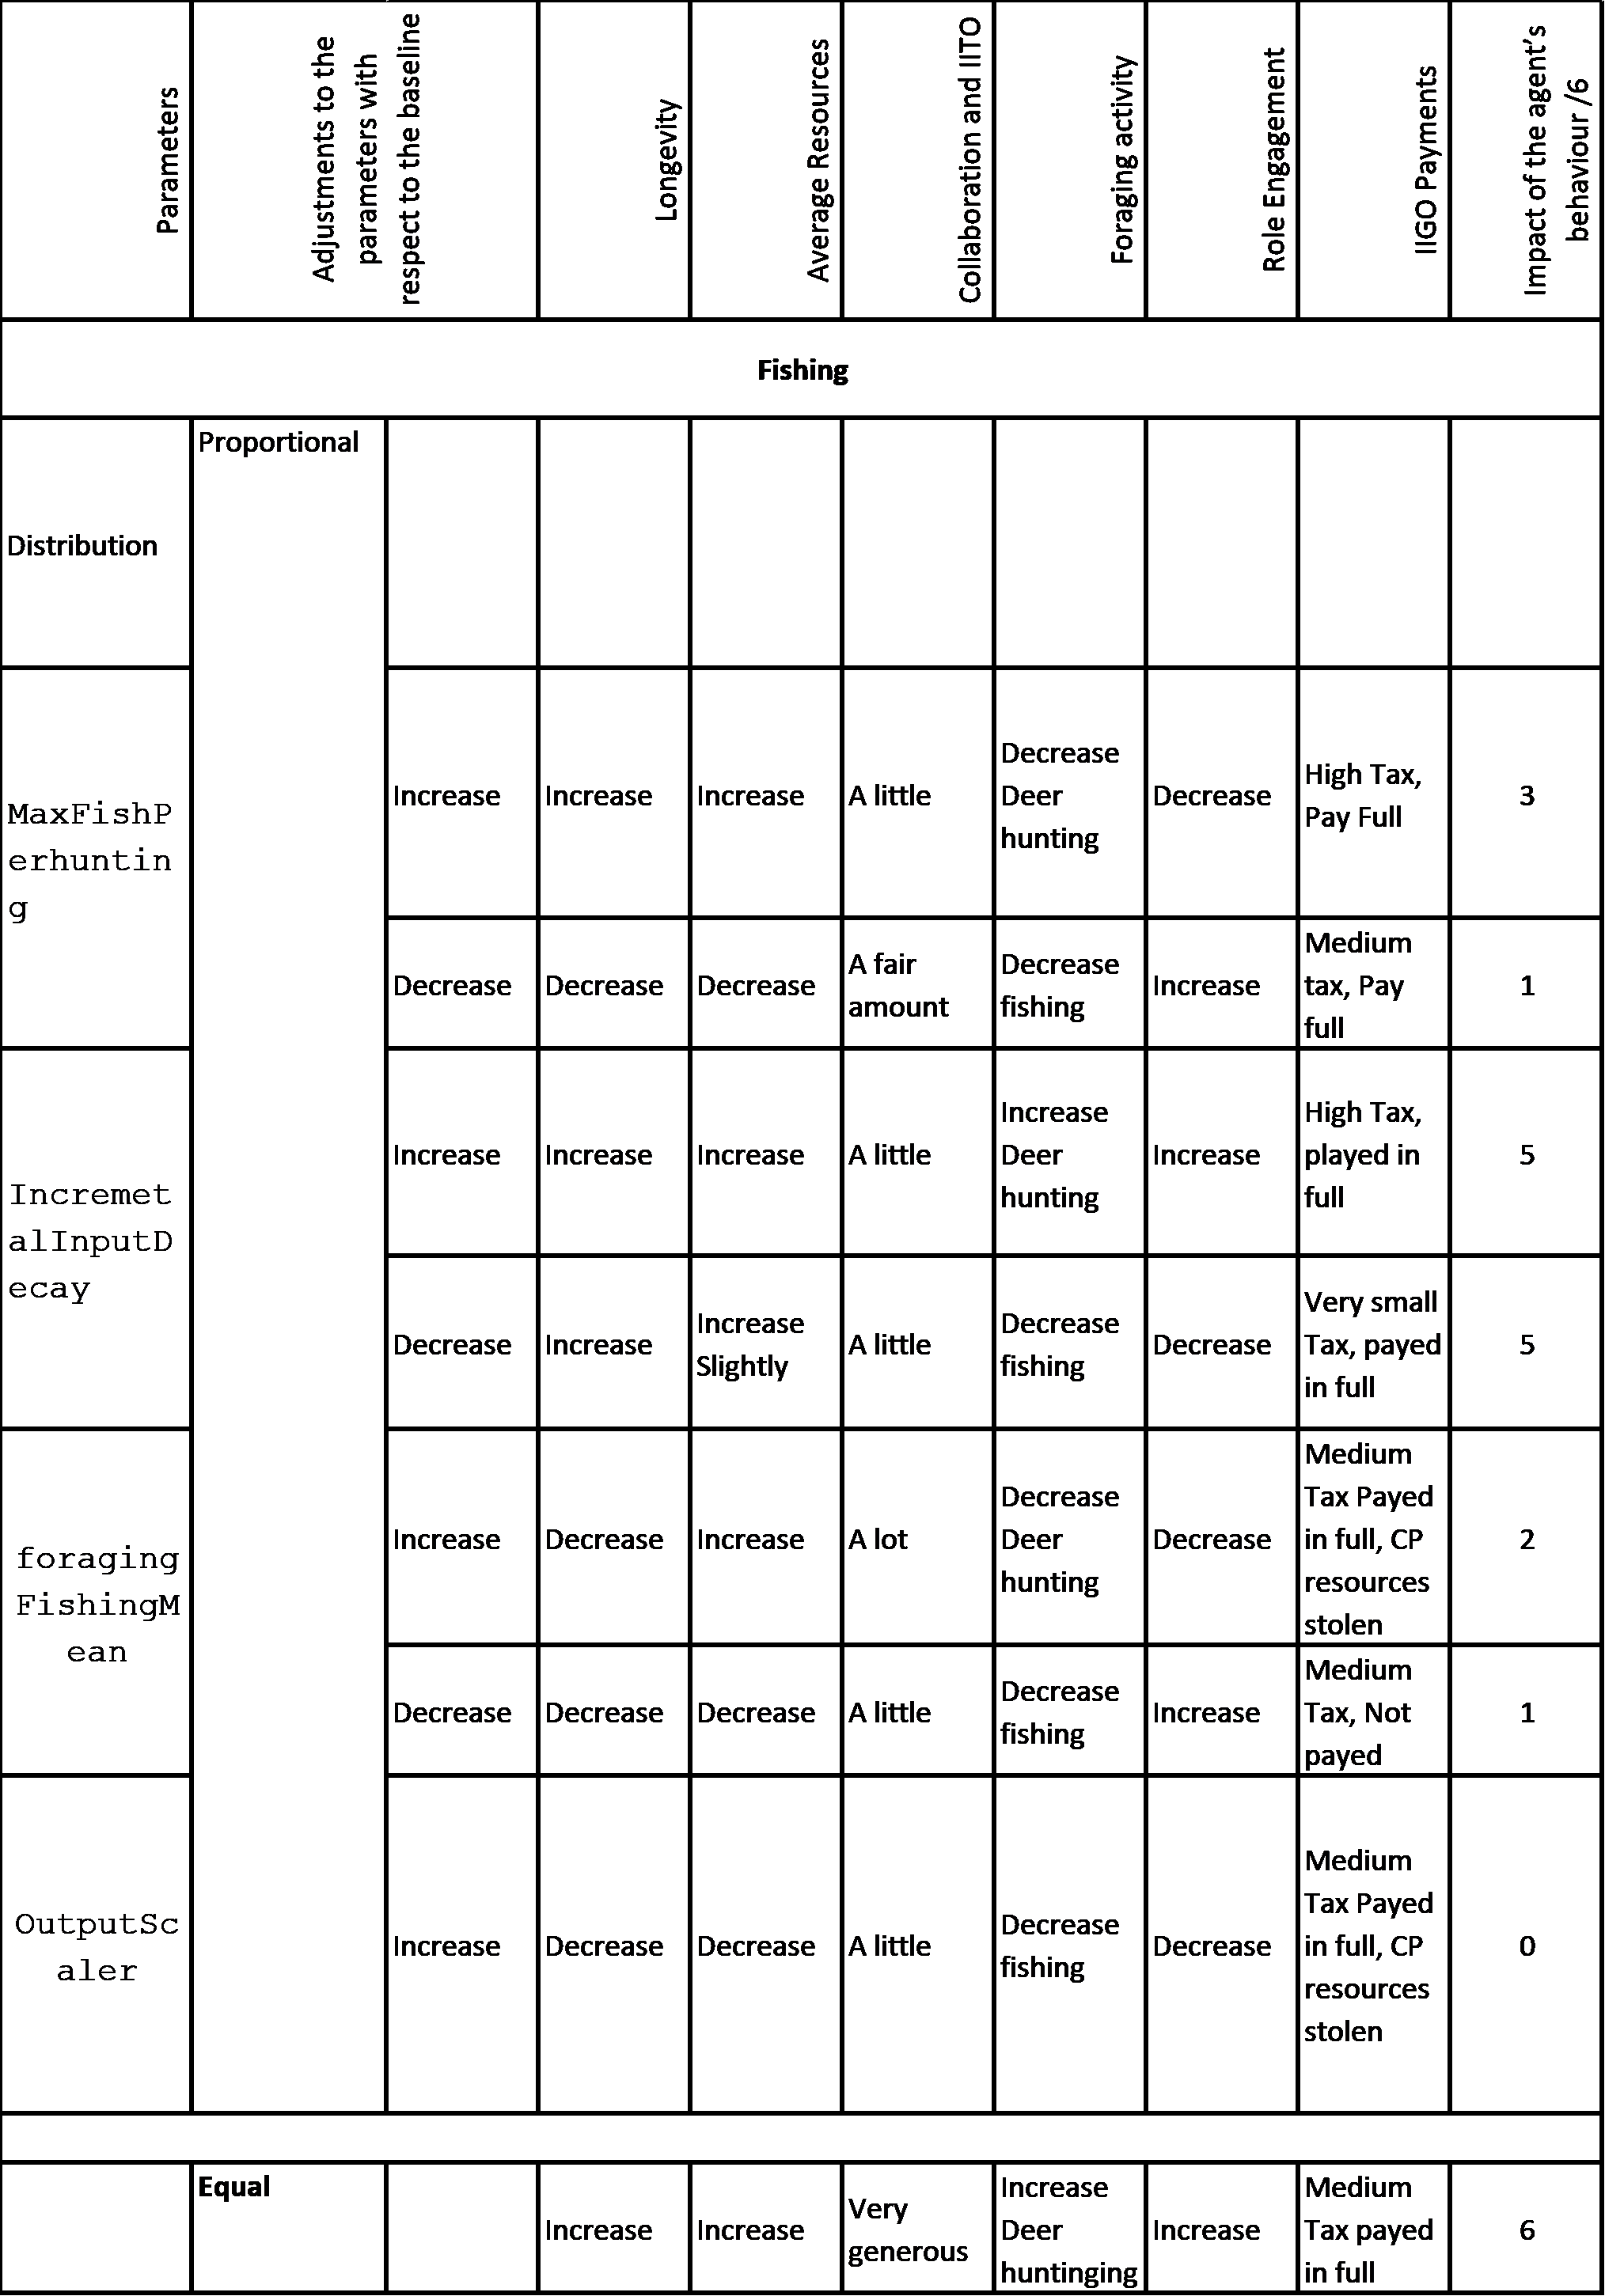
\includegraphics[width=0.8\textwidth]{13_team5_agentdesign/images/Foarging Simulation Fishing.png}
    \caption{Foraging Fishing parameters Simulation Results}
    \label{fig:Foraging Fishing parameters Simulation Results}
\end{figure}

\texttt{MaxFishPerHunt} parameter represents the total number of fish that can be caught in a hunt. The simulation indicates our agent's fishing efficiency increases accordingly to an increase to the parameter. However, the deer hunting efficiency is very low. Therefore, our agent has no longer an incentive to go deer hunting as he could rather go fishing, which is a more reliable foraging method and guarantees a large return.

Our agent prefers high risk high reward approach. In order to survive, our agent invests a lot of his resources into deer hunting to gain a maximum amount of resources. However, this approach proves less favourable, as the simulation uncover that our agent do not recover from the "dying" state. Therefore, the reward dominant approach is not always the optimal strategy, and the agent should learn to switch to fishing.


\subsection{Disasters}
%% Disaster
The parameters examined in Figure~\ref{fig:DisasterParams} were evaluated using metrics we devised to evaluate the effect of changes in disaster parameters. 

\begin{figure}[!htb]
    \centering
    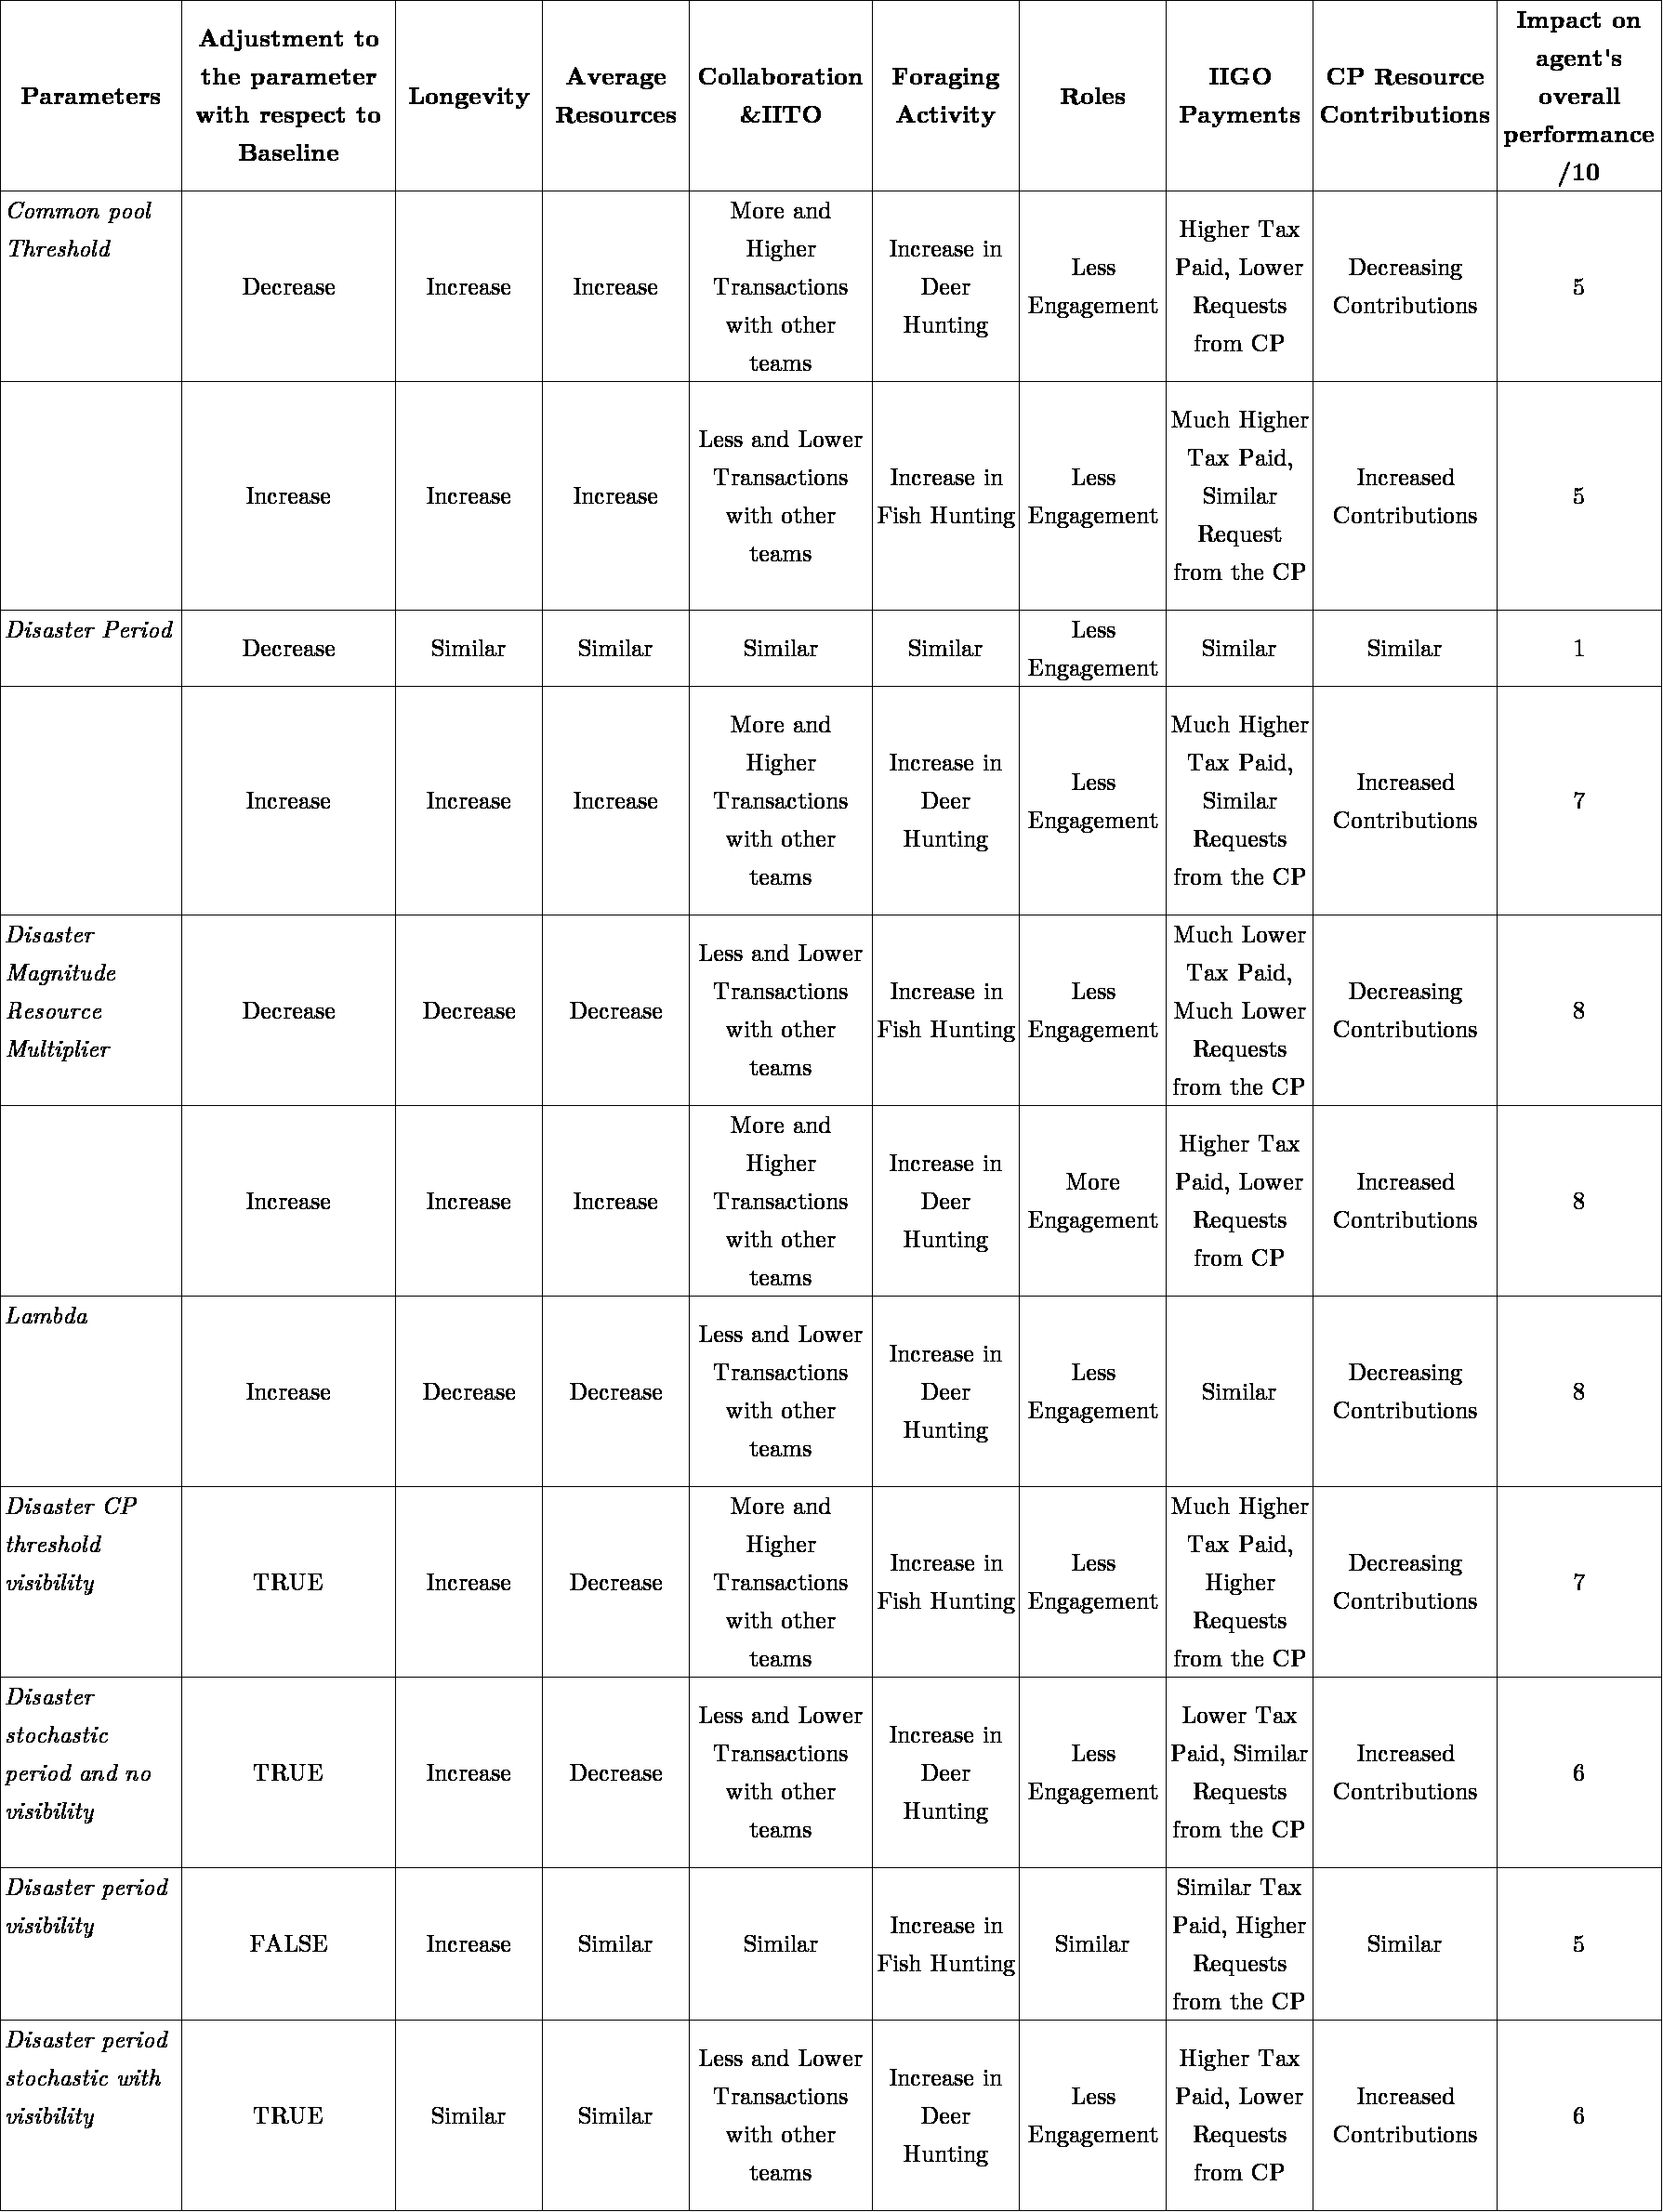
\includegraphics[width=1\textwidth]{13_team5_agentdesign/images/Sim.png}
    \caption{Exploration of Disaster Parameters on Agent Metrics}
    \label{fig:DisasterParams}
\end{figure}

The effects of varying different parameters can be visualised in 
Figure~\ref{fig:DisasterParams}, where some metrics were devised for the evaluation of our agent. Foremost, we can see that the visibility of the threshold of the Common Pool influences how our agent interacts with other agents. Particularly, it was seen that when the threshold is visible, contributions to the common pool from our agent decreased with respect to the baseline. This resulted in more and larger transactions between our agent its counterparts. This could potentially be linked to the fact that our agent determines if threshold requirements are already met before contributing. Thus, a lower common pool contribution might encourage our agent to engage in other sorts of transactions. The effect of this is maximised when the threshold is lowered, leaving more resources to spend on other sorts of agent interactions and possibly, a higher contribution to foraging. For the latter, that might not be the case as it can be seen by the decrease of average resources when common pool threshold visibility is enabled. This is likely due to the hard cap on the maximum amount that our agent can invest in foraging or possibly due to the effect of other covariate parameters on the agent's foraging decisions.

Regarding adjustments to the \texttt{disasterPeriod} parameter, it can be seen that resource contributions and interactions with other clients increase by a proportionally larger amount when disaster period increases, i.e. disasters hit less often, implying that when our agent prospers, it tends to be more generous. This is a result of its opinion formation strategy. It is important to note that under multiple simulations, when the disaster period is visible, whether that is stochastic or not, the main metric that can be seen to be affected is the contribution to the common pool. 

However if we increase the \texttt{disasterMagnitudeResourceMultiplier} it can be observed that common pool contributions either increases or stays level to the baseline parameters. At the same time, transactions seem to be decreasing, showing that our island may be entering a “defense” mode, saving up for an upcoming disaster and ensuring that the common pool threshold is met. These observations are in favour of the proposed agent functionality.

The observations made using the above parameters, are dependent on other agent’s dynamics that were implemented. Therefore, without a collective analysis of each individual agents’ performance, conclusions are limited to the observations made solely under the specified experiment. One could only effectively evaluate an agent’s dynamics, taking in mind those of the rest of the agents in the community, given that they differ. Therefore, in future work simulations could be made with a community of only Team 5’s agent instances. Else, one would need to cross-reference the results from individual agent simulations, as well as results of simulating and evaluating the community as a whole. 

\subsection{Resource Management}

In the following experiments, we are testing the amount of the resources of our agent throughout the game. For each experiment, we were keeping all the parameters fixed to baseline and adjusting only one to analyse it would affect our agent overtime. 

\underline{Parameter:} Initial Common Pool \newline
\underline{Agent Baseline Value:}1000 \newline
\underline{Tested values:} \{120, 2000, 0, 200\} \newline
\underline{Observation:} \newline
We have observed that our agent performs better in comparison to the rest when the amount of resources in the common pool is limited. This is because our agent's behaviour is not competitive and it does not request great amounts of resources if its state is not critical, while other agents often seem to exploit the common pool. An exceptional scenario is when the initial resources are too low and the agents does not manage to recover from the first disaster.
Below, there are two Figu that are representative of our agent's performance in comparison to the other agents when initial common pool is high and when it is low.

\begin{figure}[!htb]
    \centering
    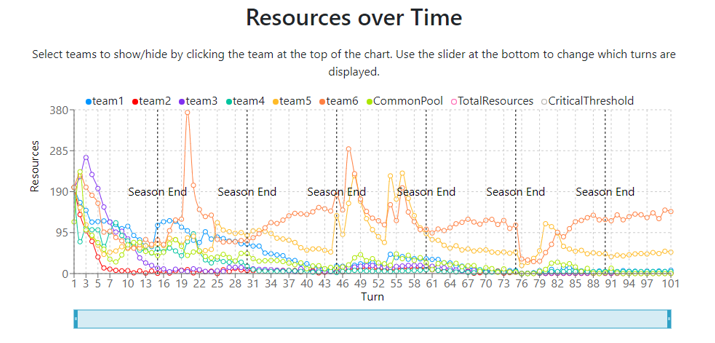
\includegraphics[width=0.6\textwidth]{13_team5_agentdesign/images/InitCP120.PNG}
    \caption{Initial Common Pool: 120}
    \label{eq:Initial Common Pool: 120}
\end{figure}

\begin{figure}[!htb]
    \centering
    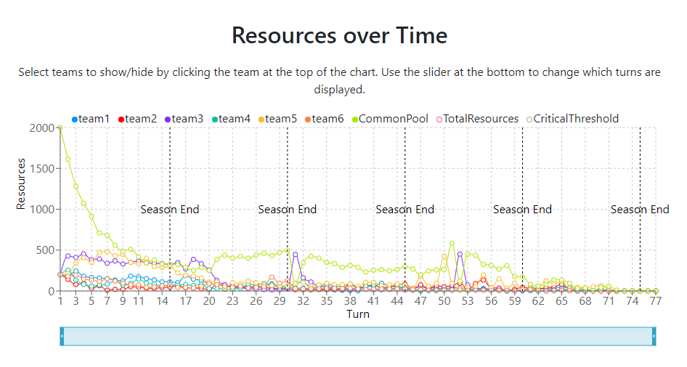
\includegraphics[width=0.6\textwidth]{13_team5_agentdesign/images/InitCP2000.PNG}
    \caption{Initial Common Pool: 200}
    \label{Initial Common Pool: 200}
\end{figure}

\underline{Parameter:} Initial Resources \newline
\underline{Agent Baseline Value:}200 \newline
\underline{Tested values:} \{50, 500, 1000\} \newline
\underline{Observation:} \newline
What was observed in these experiments is that our agent is ignorant to the initial amount of resources. More specifically, no matter what the initial resources, our agent's resource level stabilises after some number of turns. Our agent is designed to have a sophisticated foraging strategy and thus, its survival does not depend on the given resources or the common pool. The graph below illustrates this.

\begin{figure}[!htb]
    \centering
    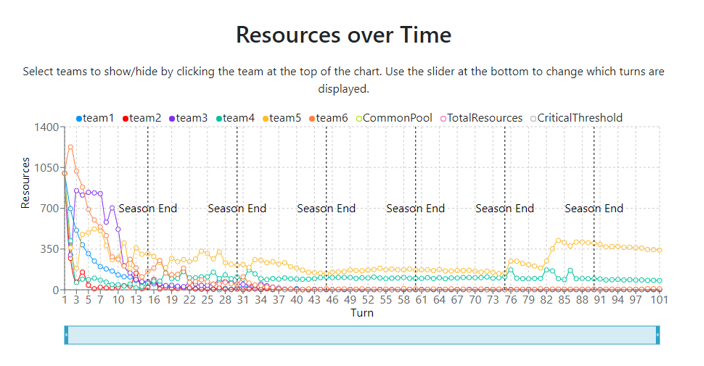
\includegraphics[width=0.6\textwidth]{13_team5_agentdesign/images/InitRes.PNG}
    \caption{Initial Resources of agent: 1000}
\end{figure}


\underline{Parameter:} Cost of Living \newline
\underline{Agent Baseline Value:}5 \newline
\underline{Tested values:} \{100, 50, 1, 10\} \newline
\underline{Observation:} \newline
The results of these experiments where similar to the ones of the previous experiment. Our agent survives and arrives in a state of equilibrium independently of the cost of living, as long as it is not extremely high; $\approx$ 100.

\underline{Parameter:} Maximum Number of Turns \newline
\underline{Agent Baseline Value:}100 \newline
\underline{Tested values:} \{200, 300\} \newline
\underline{Observation:} \newline
In this trial, our aim was to test the longevity of our agent. We observed that in all the experiments our agent managed to remain alive. Following to what has been described above, our agent develops a sustainable strategy that assures its survival and persistence. Additionally to that, we observed that after the leave of some agents, the whole environment becomes more stable and the remaining agents manages to maintain a fixed amount of resources. A possible explanation could be that the environmental parameters such as available resources etc. are not sufficient to satisfy six islands.
\newline
\textit{Note: We also tested multiple combinations of the values of the parameters \texttt{minimumResourceThreshold} and \texttt{maxCriticalConsecutiveTurns} but since our agent manages to maintain a sufficient amount of resources throughout all the turns of the baseline scenario, it is not affected by these parameter - as long as they remain in a reasonable value.}

















\subsection{Discussion}

Overall, our agent has a set of different actions to take depending on how other islands interact with it. It is interesting to see how the agent's behavior constantly changes in simulations even without any change in the game's parameters.Given more time, it would be interesting to incorporate personality behaviour such as altruistic and selfish according to our wealth tiers. Furthermore having these internal personalities change as the game progresses or when certain roles are achieved. 



%\section{\appendixautorefname{}}
%\lstinputlisting[language=go]{configbaseline.go}




